% !TEX TS-program = xelatex
\documentclass[12pt,a4paper,twoside]{book}
\usepackage[T1]{fontenc}
\usepackage[english]{babel}
\usepackage{amsmath}
\usepackage{amsfonts}
\usepackage{amssymb}
\usepackage{graphicx}
\usepackage[hidelinks]{hyperref}
\usepackage{wrapfig}
\setlength\columnsep{1em}

\usepackage[margin=1in]{geometry}

\usepackage{xfrac}

\usepackage{siunitx}
\sisetup{quotient-mode=fraction, fraction-function=\sfrac,
	product-units = single,output-product={\,}, % We are abusing product to get nice fractions
	range-phrase=--,range-units=single}
\DeclareSIUnit\inch{in}
\DeclareSIUnit\pound{lb}
\DeclareSIUnit\teaspoon{tsp}
\DeclareSIUnit\tablespoon{tbsp}
\DeclareSIUnit\cup{cup}
\DeclareSIUnit\ounce{oz}
\DeclareSIUnit\flounce{fl oz}
\DeclareSIUnit\fahrenheit{\degree F}

\usepackage{xcookybooky}
\setlength{\headheight}{15pt}
\setRecipeColors{%
    recipename = black,
    numeration = black}
\setRecipeSizes{%
    recipename = \Huge,
    inghead = \large,
    prephead = \large}
\setRecipeLengths{%
    ingredientswidth = 0.45\textwidth}
% https://tex.stackexchange.com/questions/68745/possible-values-for-fontseries-and-fontshape
% "Helvetica", T1 encoding, bold weight, normal shape
\setRecipenameFont{qhv}{T1}{b}{n}
% https://tex.stackexchange.com/questions/481698/missing-endcsname-in-package-xcookybooky-texlive
\renewcommand{\step}
{%
 \stepcounter{step}%shouldn't be in the argument of lettrine
    \lettrine
    [%
        lines=2,
        lhang=0,          % space into margin, value between 0 and 1
        loversize=0.15,   % enlarges the height of the capital
        slope=0em,
        findent=1em,      % gap between capital and intended text
        nindent=0em       % shifts all intended lines, begining with the second line
    ]{\fontfamily{lmr}\selectfont\thestep}{}%
}

%
% Need this for wide latin
%
\usepackage{fontspec}
\setmainfont{XCharter}
\setsansfont{TeX Gyre Heros}
\newfontfamily{\japanesefont}{Ume Mincho}
\newfontfamily{\scripterfont}{QTArtiston}
\usepackage[CJK]{ucharclasses}
\setTransitionsForJapanese{\japanesefont}{}


\title{Recipes}
\author{\texttt{chemistring}\\%
		\texttt{chimingfish}\\%
		\texttt{ekimekim}\\%
		\texttt{HeNine}\\%
		\texttt{Hiramas}\\%
		\texttt{HubbeKing}\\%
		\texttt{LambMower}\\%
		\texttt{Lunik}\\%
		\texttt{mithodin}\\%
		\texttt{Roosevelt}
}

\begin{document}
	\maketitle
	\tableofcontents
	\clearpage

	\chapter{The Recipes}

	\begin{recipe}
[ %
        preparationtime = {\SI{20}{\hour}},
        bakingtime={\SI{1}{\hour}},
        bakingtemperature={\protect\bakingtemperature{topbottomheat=\SI{280}{\celsius}}},
        portion = {\portion[Loaf]{1}},
        source = {Hiramas}
    ]{Hirabread}
	    
	    \begin{figure}[p]
	        \centering
	        \makebox[\textwidth][c]{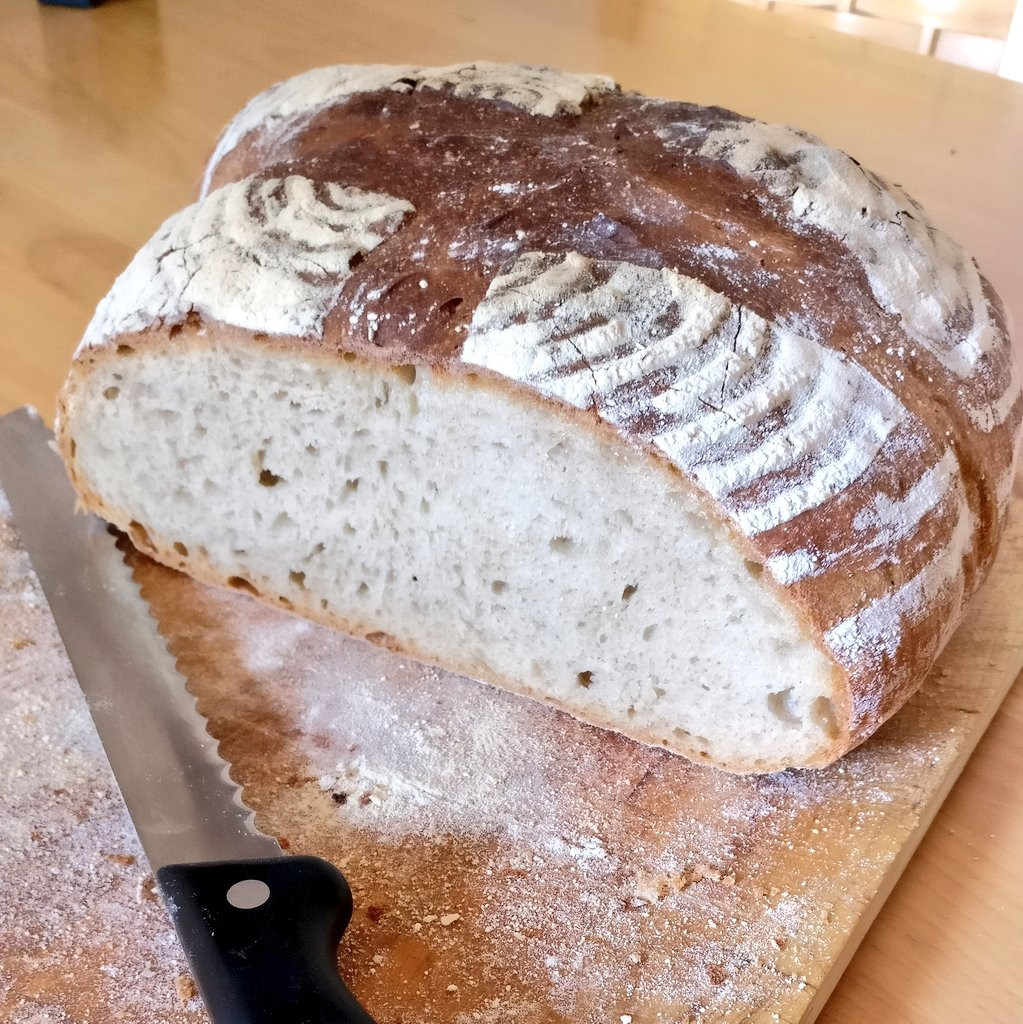
\includegraphics[height=\textheight]{hirabread/EV0I-6cUcAkaNUL.jpg}}
	    \end{figure}
	    
		\ingredients[14]{
		    \multicolumn{2}{c}{\textbf{Rye preferment}} \\
		    \SI{120}{\gram} & Rye flour 1150 \\
		    \SI{100}{\gram} & Water \\
		    \SI{8}{\gram} & Starter \\
		    & \\
		    \multicolumn{2}{c}{\textbf{Wheat preferment}} \\
		    \SI{75}{\gram} & Wheat flour 550 \\
            \SI{75}{\gram} & Water \\
            \SI{0.1}{\gram} & Fresh baker's yeast \\
            & \\
            \multicolumn{2}{c}{\textbf{Main dough}} \\
            \SI{375}{\gram} & Wheat flour 1050 \\
            \SI{125}{\gram} & Wheat flour 550 \\
            \SI{13}{\gram} & Salt \\
            \SI{6}{\gram} & Fresh baker's yeast \\
            \SI{300}{\gram} & Water 
		}
		
		\preparation {
		    \step Mix the rye dough and let ferment for \SI{18}{\hour} at a falling temperature, from \SIrange{30}{20}{\celsius}.
		    \step Mix the wheat dough and let ferment for \SI{18}{\hour} at \SI{20}{\celsius}.
		    \step Knead the dough and rest for \SI{45}{\minute} at \SI{24}{\celsius}.
		    \step Shape the dough, let rest for \SI{50}{\minute} at \SI{24}{\celsius}.
		    \step Bake the dough, with seam down, and scored with a cross, starting at \SI{280}{\celsius}, falling to \SI{200}{\celsius} for \SI{60}{\minute}.
		}
\end{recipe}
    \clearpage
	\begin{recipe}
[ %
        preparationtime = {\SIrange{3}{5}{\hour}},
        portion = {\portion{4--5}},
        source = {HeNine}
    ]{Goulash}

        \begin{figure}[p]
	        \centering
	        \makebox[\textwidth][c]{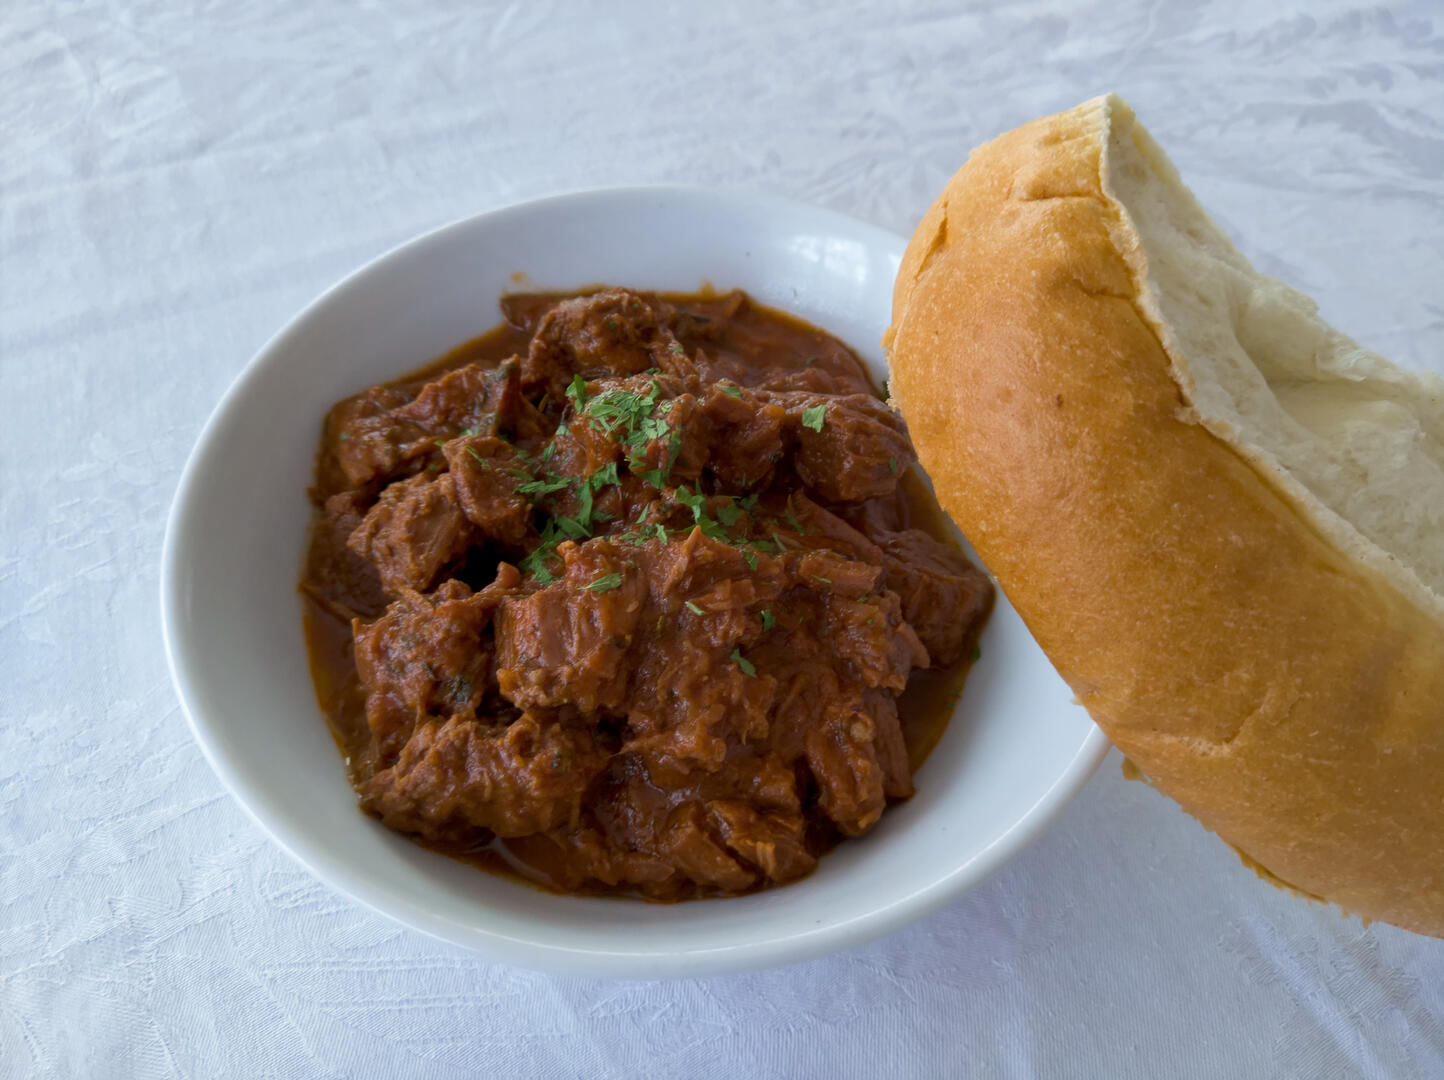
\includegraphics[height=\textheight]{goulash/IMG_20200202_120631.jpg}}
	    \end{figure}

	    \introduction{%
	        \textbf{\large BEEF}

	        Use a cheaper cut of meat, like thigh, flank or shoulder. You'll be stewing it to soften and adding lots of spices to maximize the taste.

            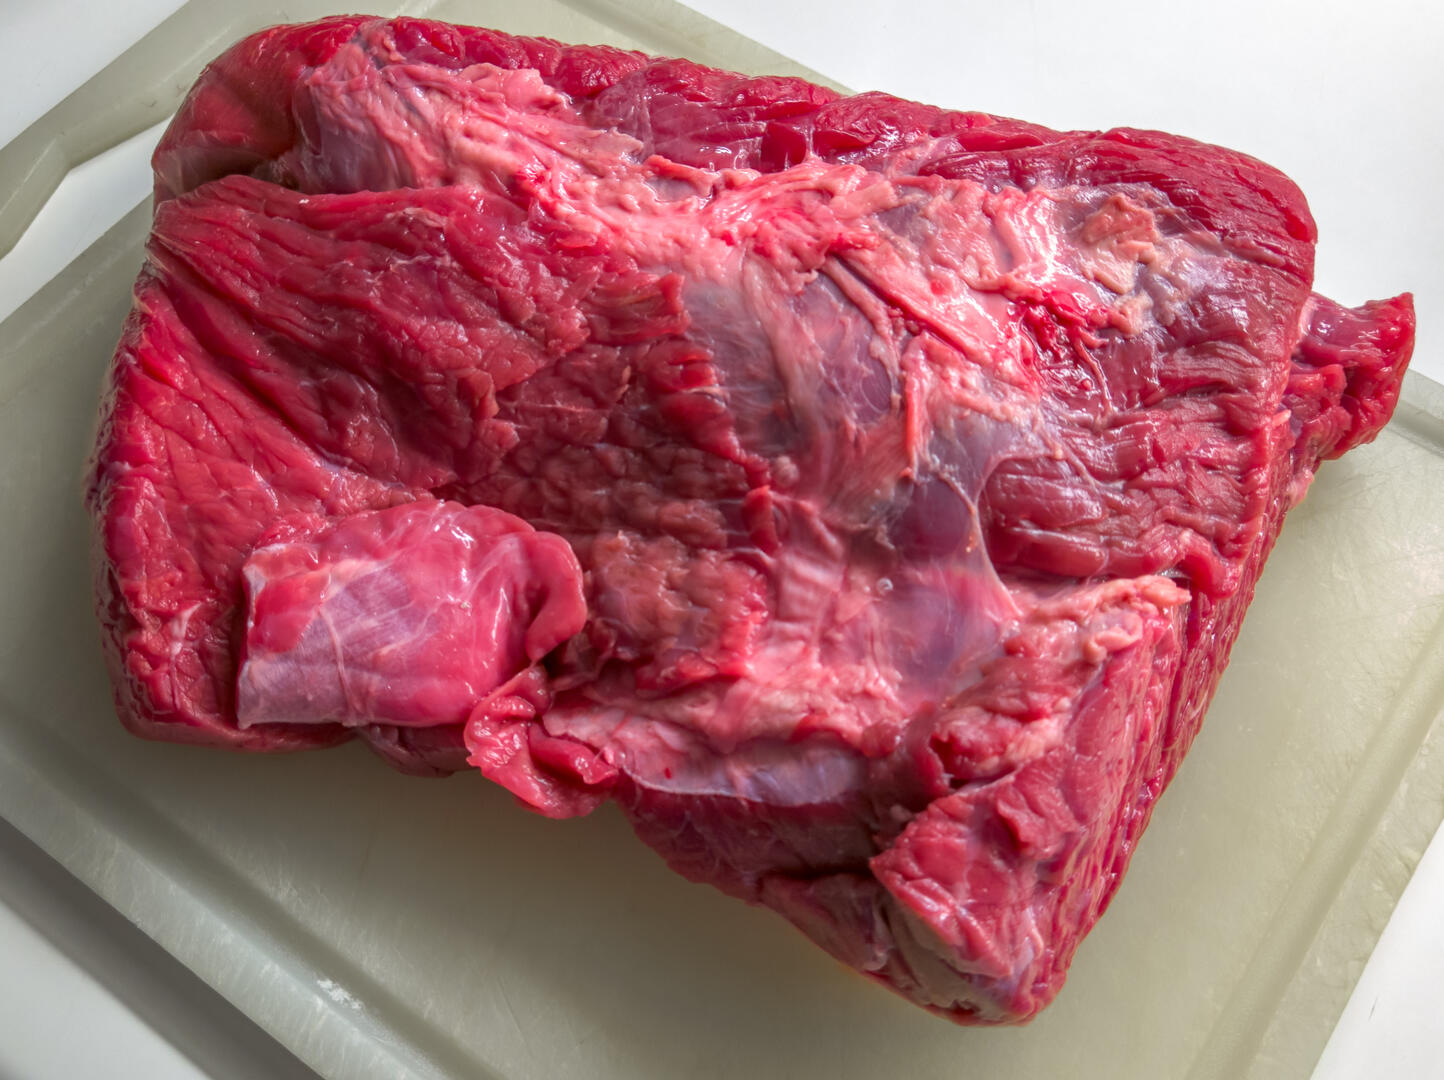
\includegraphics[width=\textwidth]{goulash/IMG_20200202_084818.jpg}

            \textbf{\large Onion}

            This is a pretty flexible recipe. You can use anywhere between 0.3 and 1.5 kg (per 1 kg of meat). I like a meatier version and onions make me farty.

            You can also use red or white or yellow onions OR A MIX! Fuck this boi up with onions!

            \newpage
            \textbf{\large Spice mix}

            The amounts here are eyeballed and I tend to go easy on cumin, but this mix works for me.

            Because we stew the meat for a long time I try to leave the herbs and spices in larger chunks: whole juniper berries, whole bay leaf, whole peppercorns, whole slightly crushed garlic cloves; I haven’t tried whole cumin and caraway, but that should also work.

            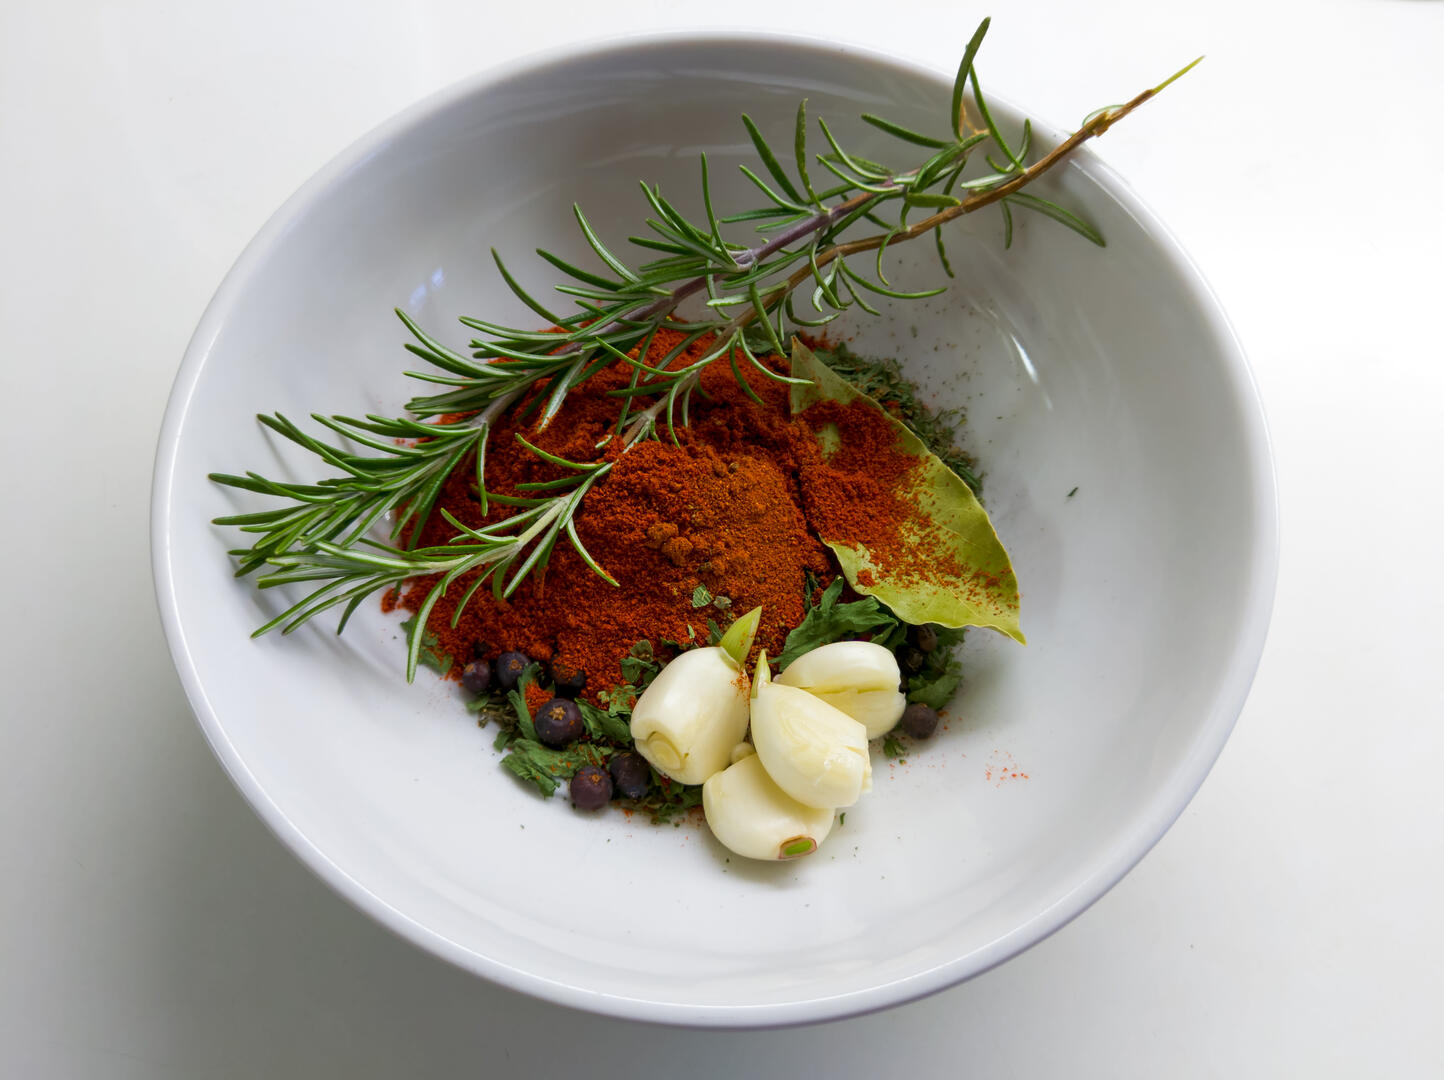
\includegraphics[width=0.5\textwidth]{goulash/IMG_20200202_095145.jpg}%
            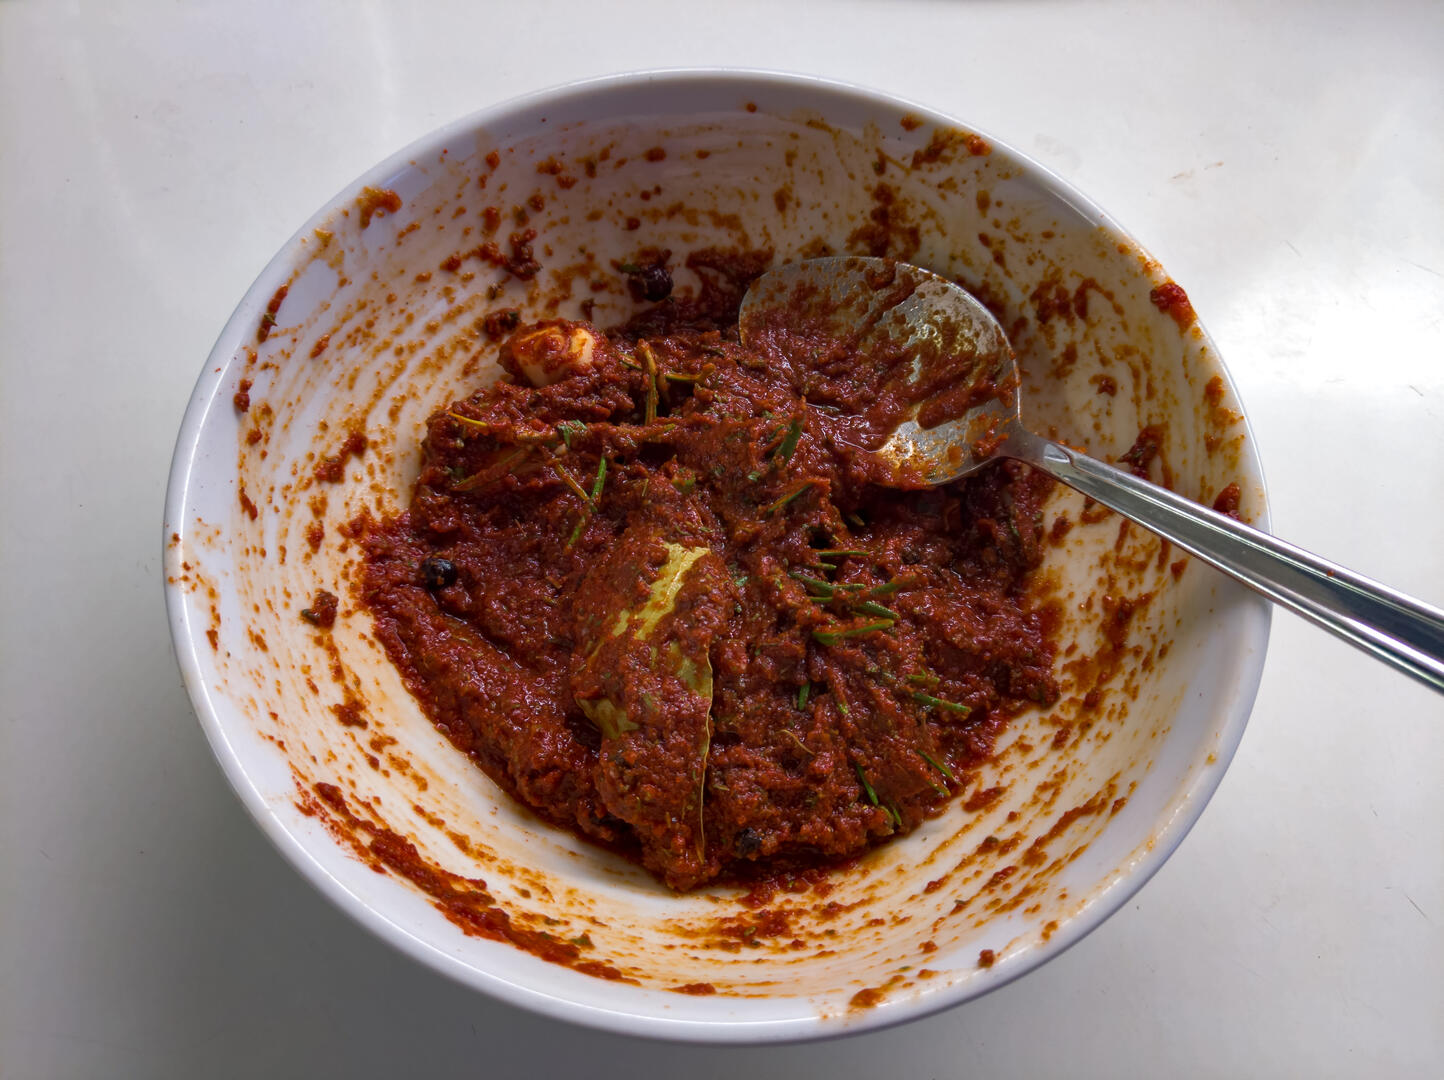
\includegraphics[width=0.5\textwidth]{goulash/IMG_20200202_095816.jpg}

            I pre-mix the spices with the tomato pur\'ee and the salt before adding them to the pot: mostly because I like how it looks and also to have something to do while the meat is browning.
	    }

	    \ingredients[16]{
            \SI{1}{\kilo\gram} & BEEF \\
            \SI{0.3}{\kilo\gram} & Onion \\
            1\,tsp & Thyme \\
            1\,tsp & Dry celery leaves \\
            1\,tsp & Summer savory (is apparently what it’s called) \\
            1\,tsp & Marjoram \\
            0.5\,tsp & Cumin \\
            1.5\,tsp & Caraway \\
            1\,large & Bay leaf or several small bay leaves \\
            idk some & Whole peppercorns \\
            7--10 & Juniper berries \\
            1.5\,tbsp & Paprika \\
            1\,sprig & Rosemary \\
            2\,cloves & Garlic \\
            1\,mTc & Salt! \\
            2\,tbsp & Tomato pur\'ee
        }

    \preparation{

        \step Clean and cut the meat into walnut-sized qubes. You don’t have to remove all fat and connective tissue, but the more you leave the longer it will take to render and soften.

%        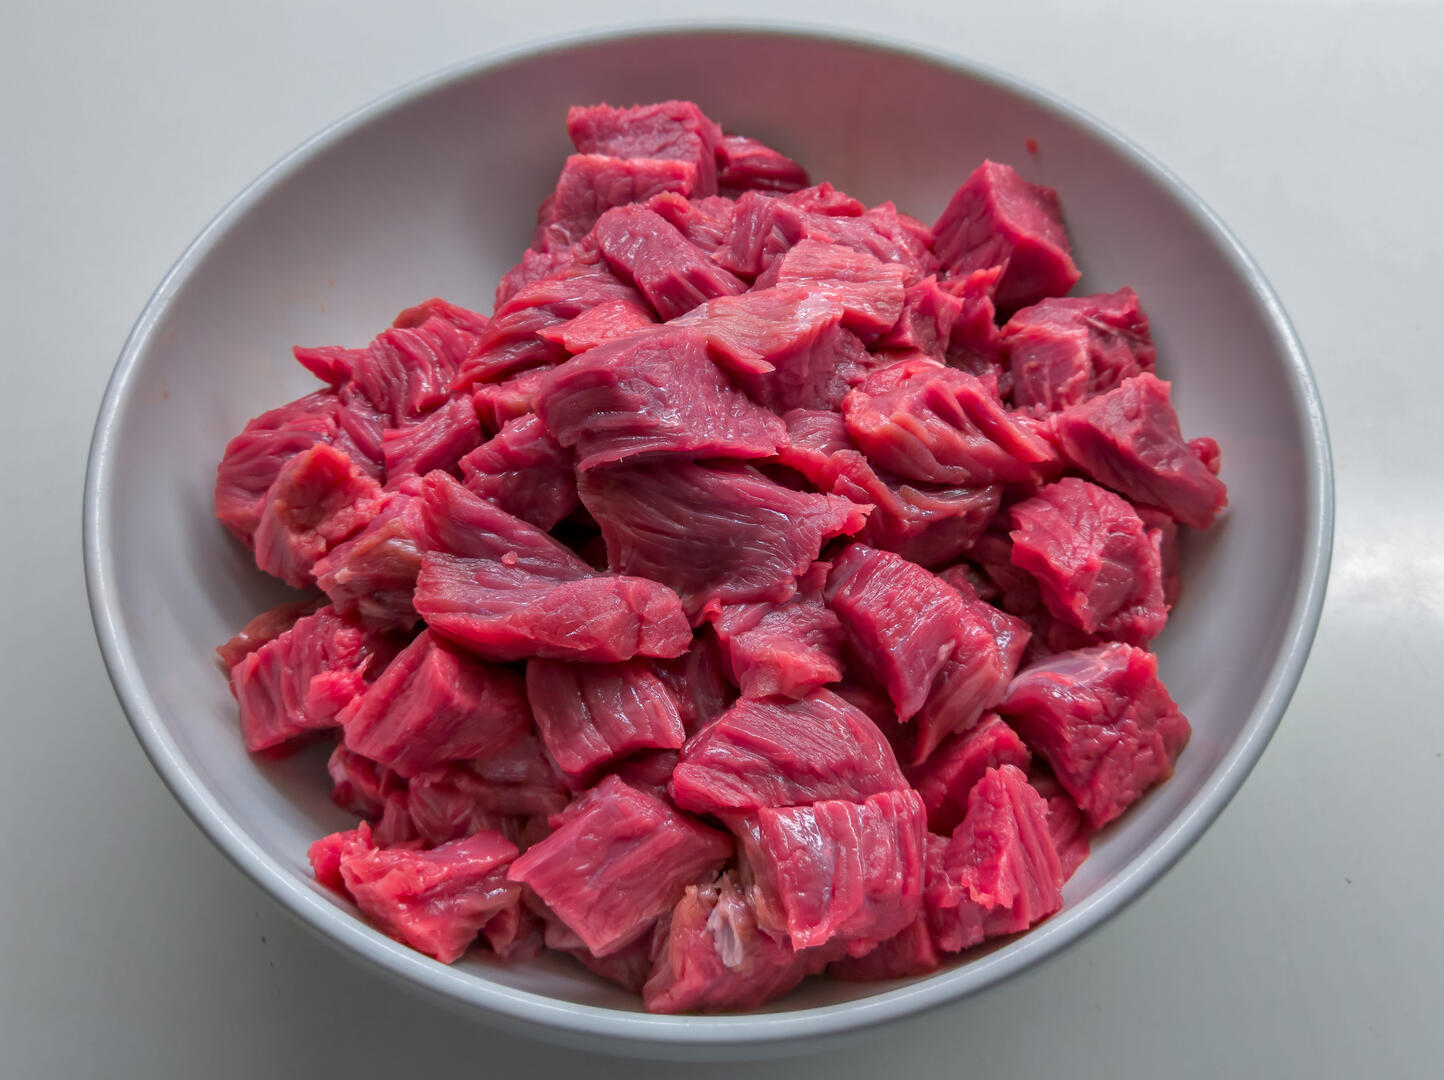
\includegraphics[width=0.53\textwidth]{goulash/IMG_20200202_091357.jpg}


        \step Slice the onions. The onions will ``melt'' while they cook, so you can chop them very roughly: small onions into quarters, larger onions lengthwise into 1 cm strips. Also, you’re cleaning and slicing like a kilogram of onions; you don’t wanna finely chop that many onions, do you?

%        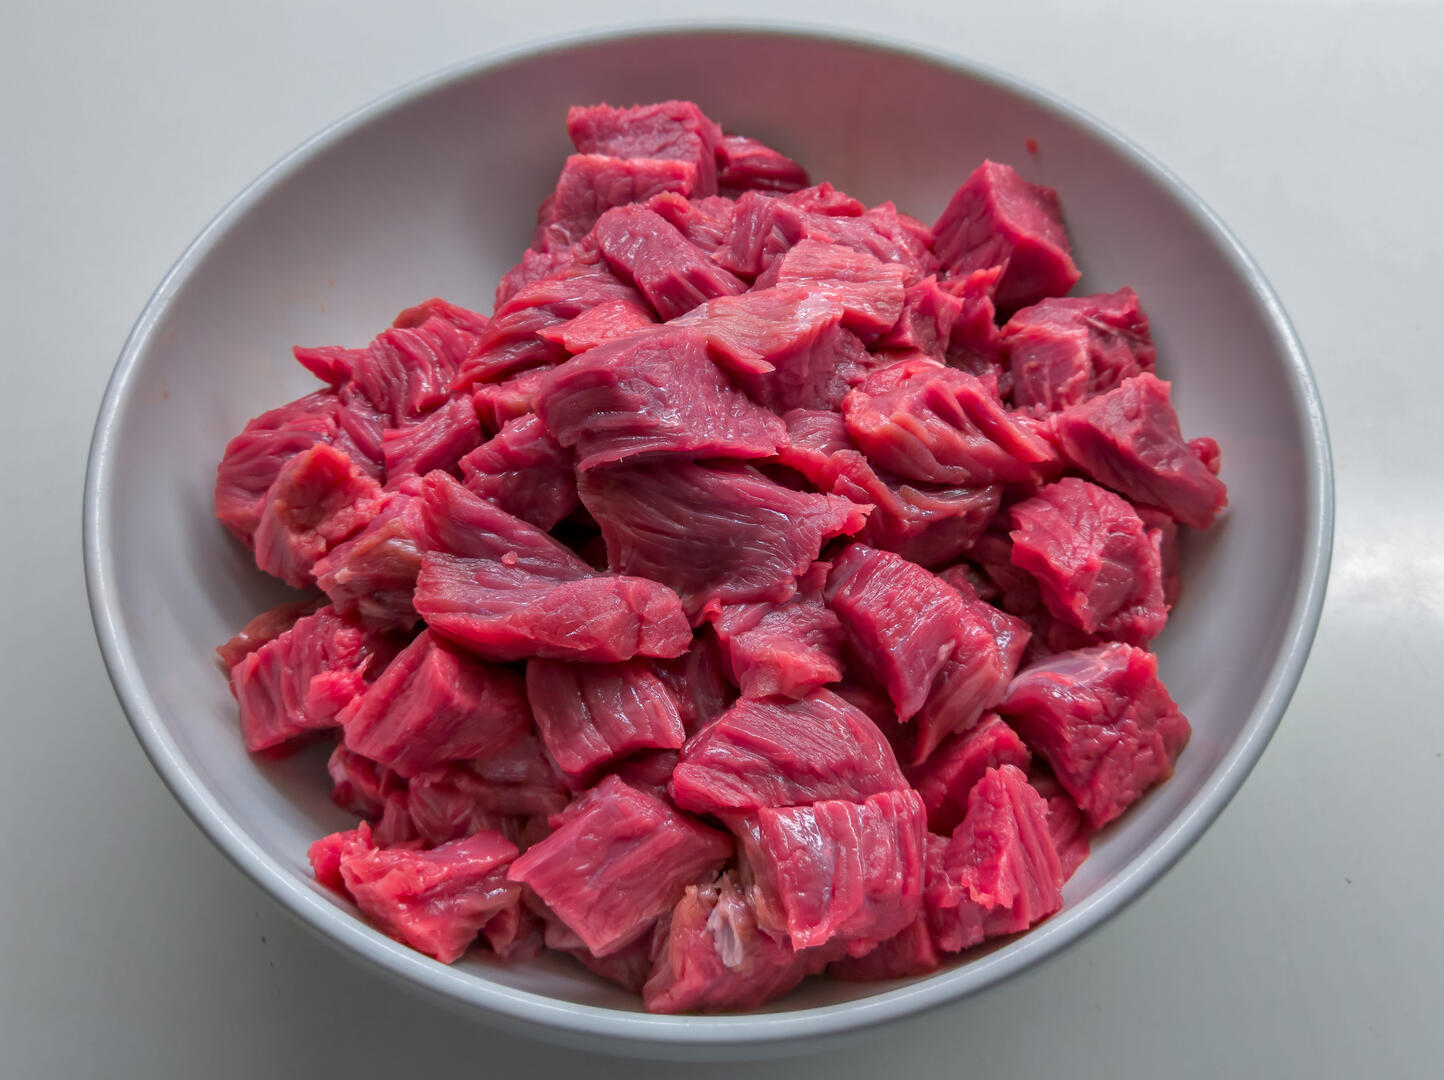
\includegraphics[width=0.5\textwidth]{goulash/IMG_20200202_091357.jpg}%
%        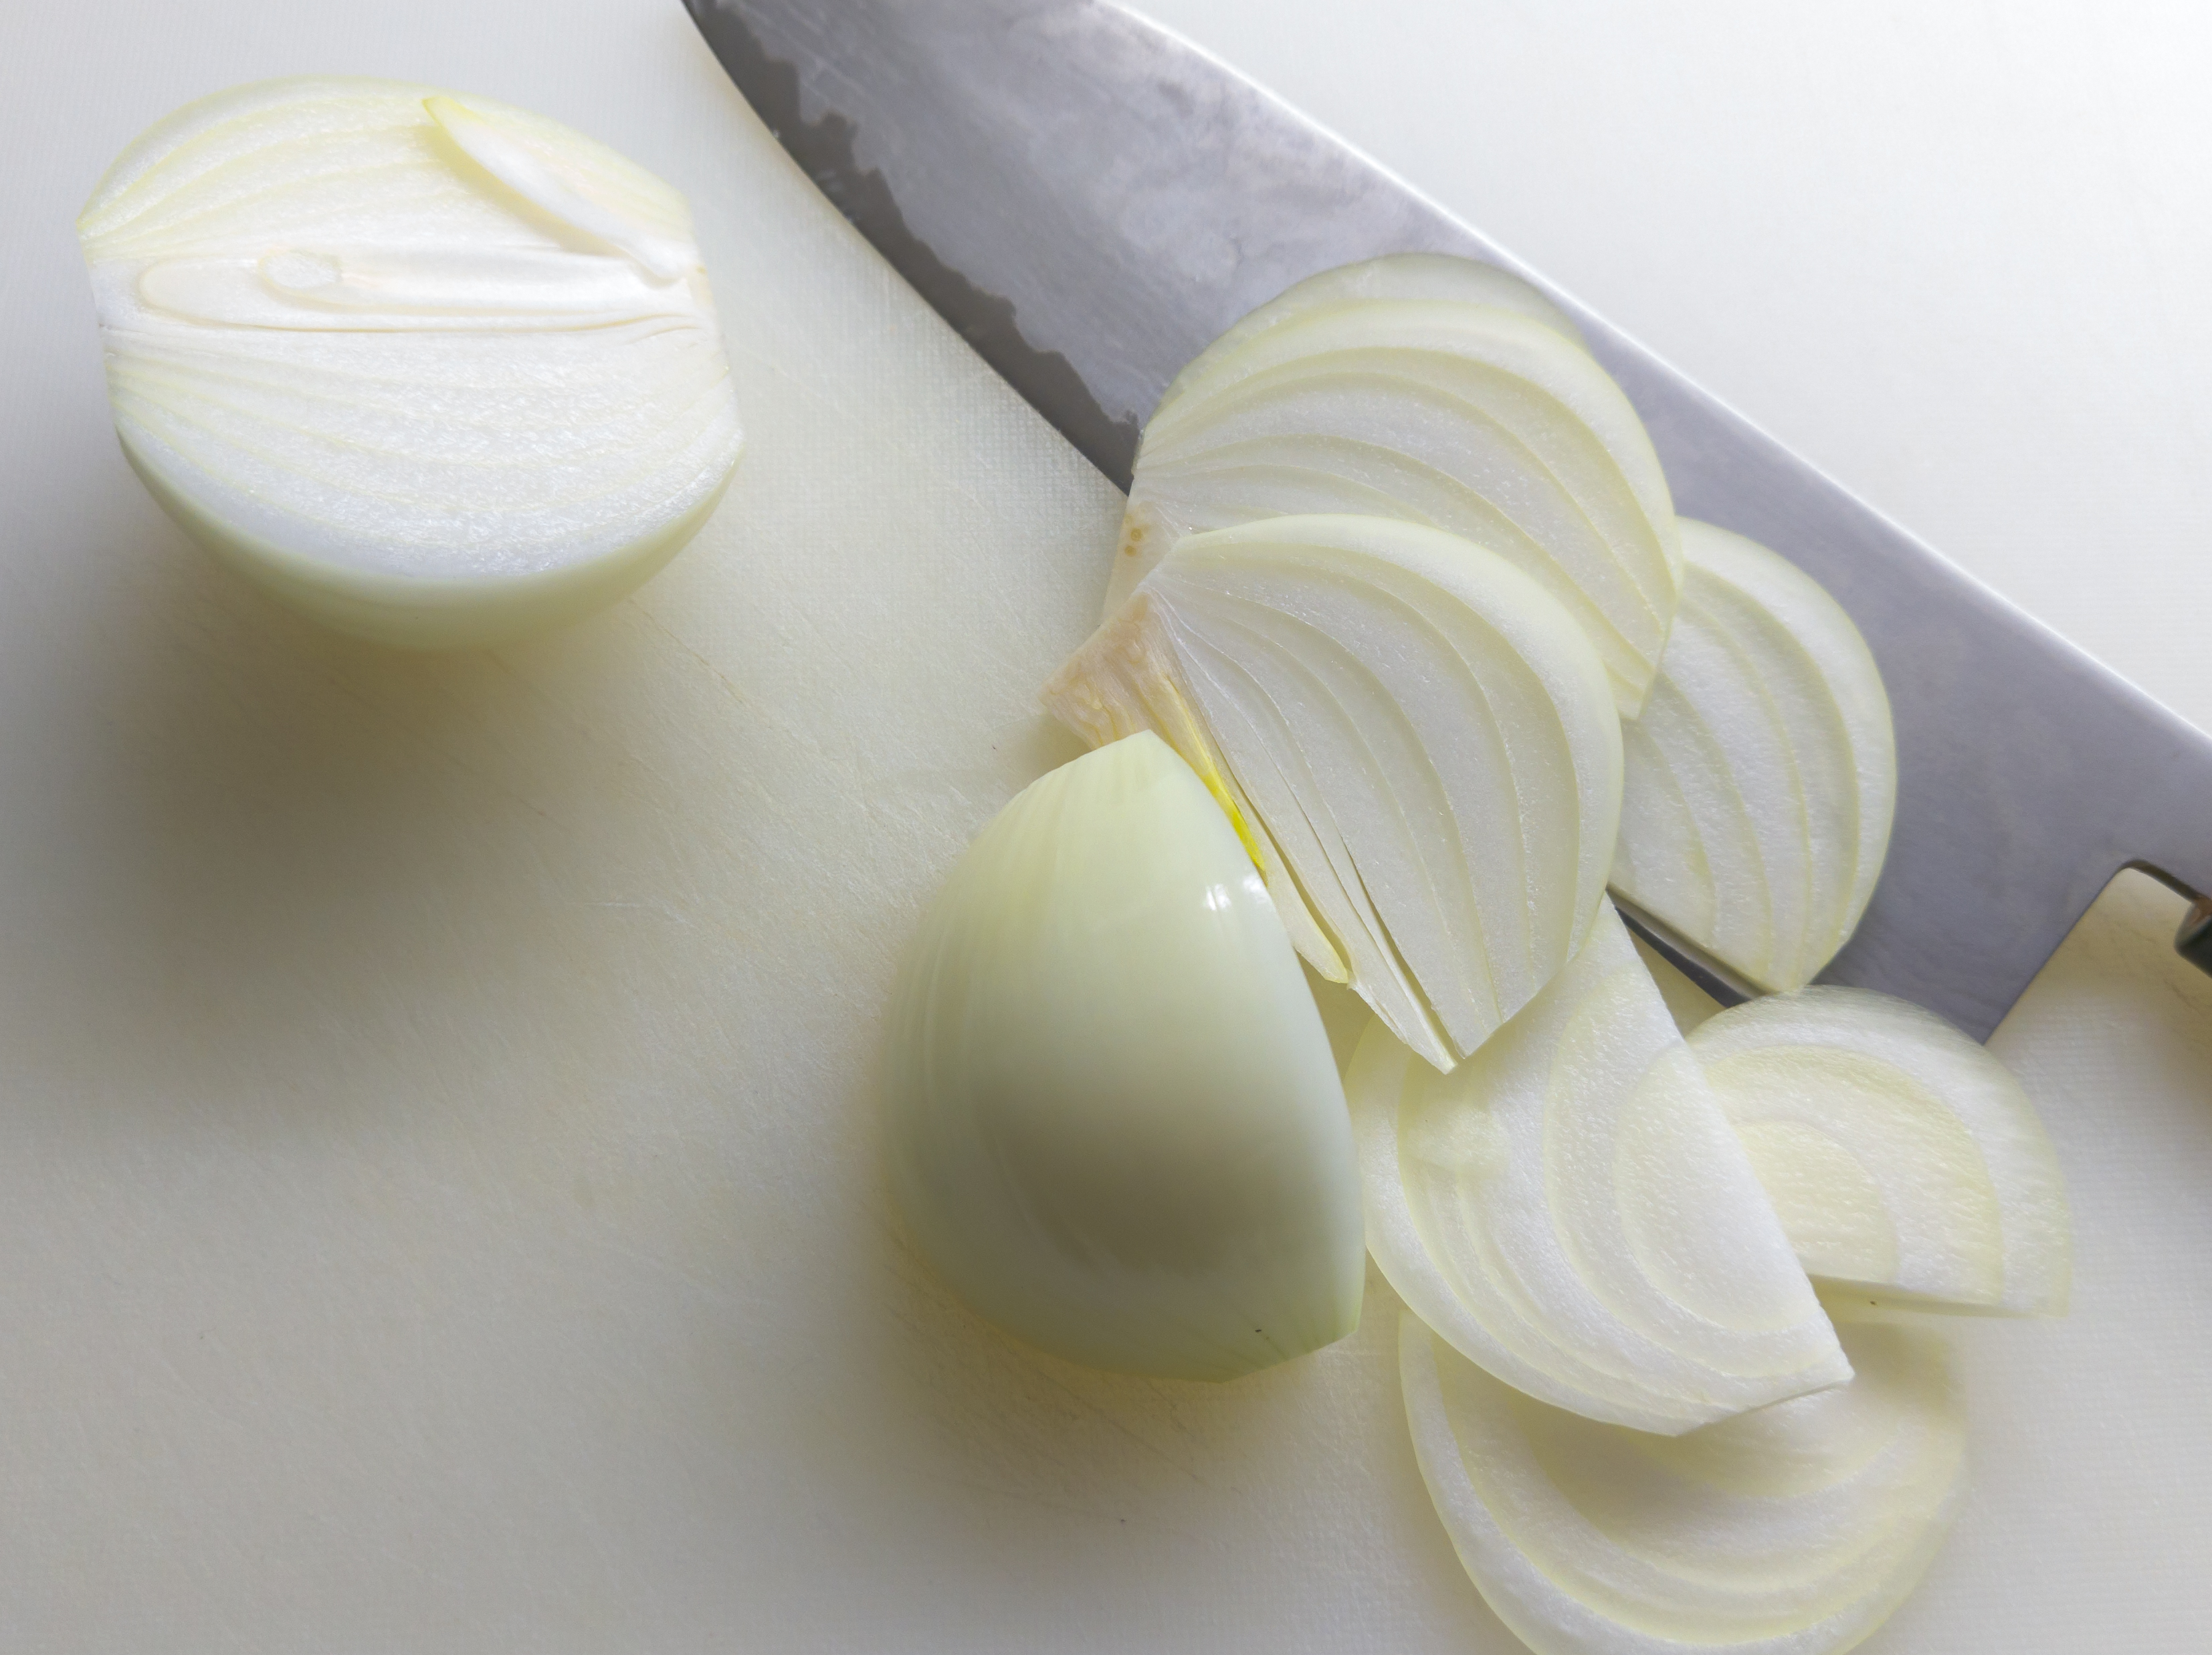
\includegraphics[width=0.5\textwidth]{goulash/IMG_20200202_091811.jpg}

%        \begin{wrapfigure}[11]{r}{0.51\textwidth}%
%            % \centering%
%            \hspace{-23pt}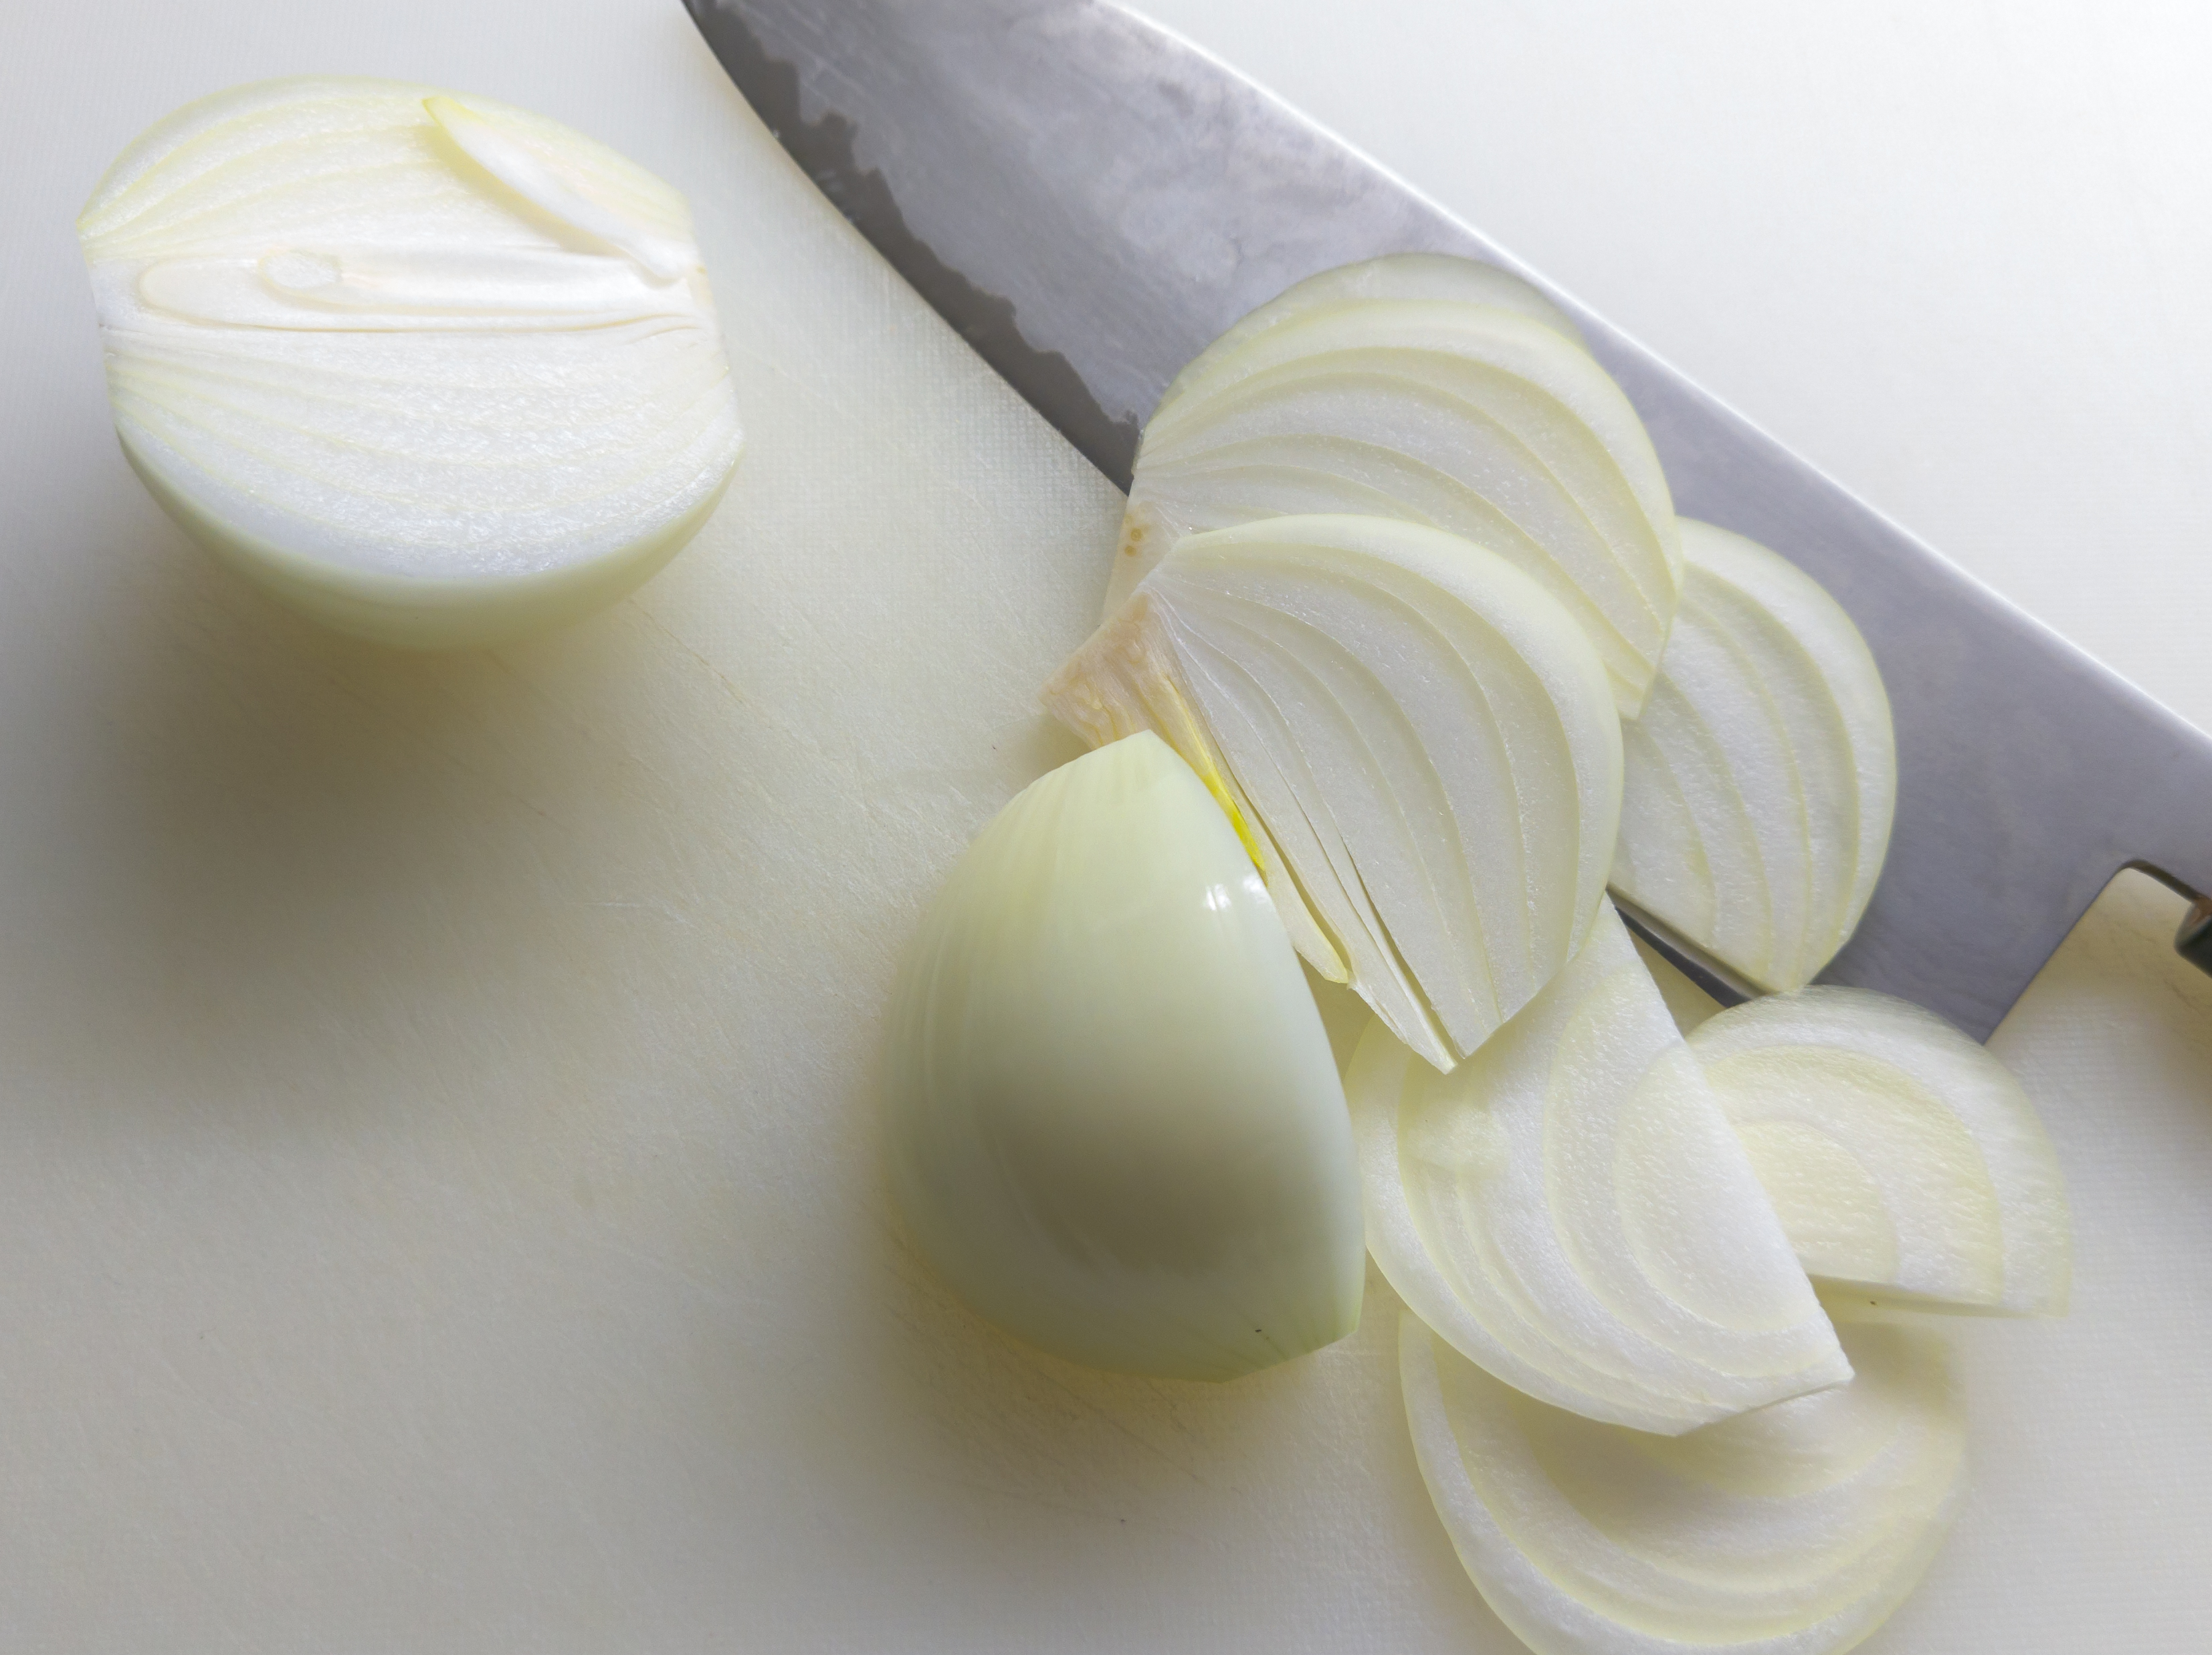
\includegraphics[width=0.5\textwidth]{goulash/IMG_20200202_091811.jpg}
%        \end{wrapfigure}

        \step Start saut\'eing the onions on high-mid heat on a bit of oil.

        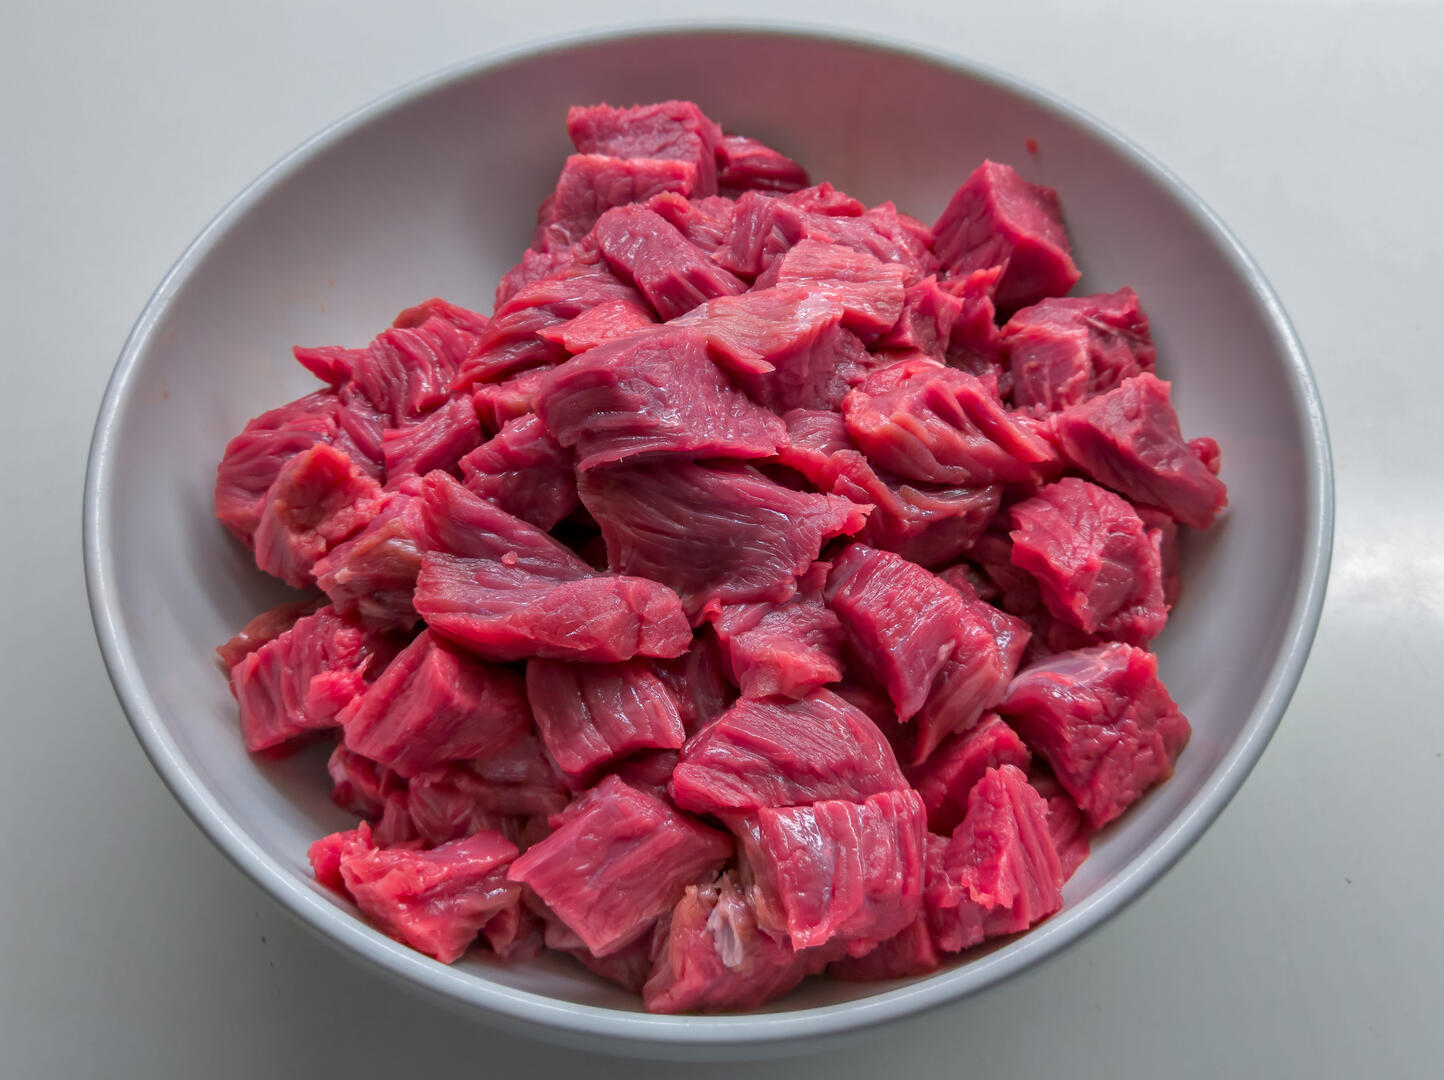
\includegraphics[width=0.5\textwidth]{goulash/IMG_20200202_091357.jpg}%
        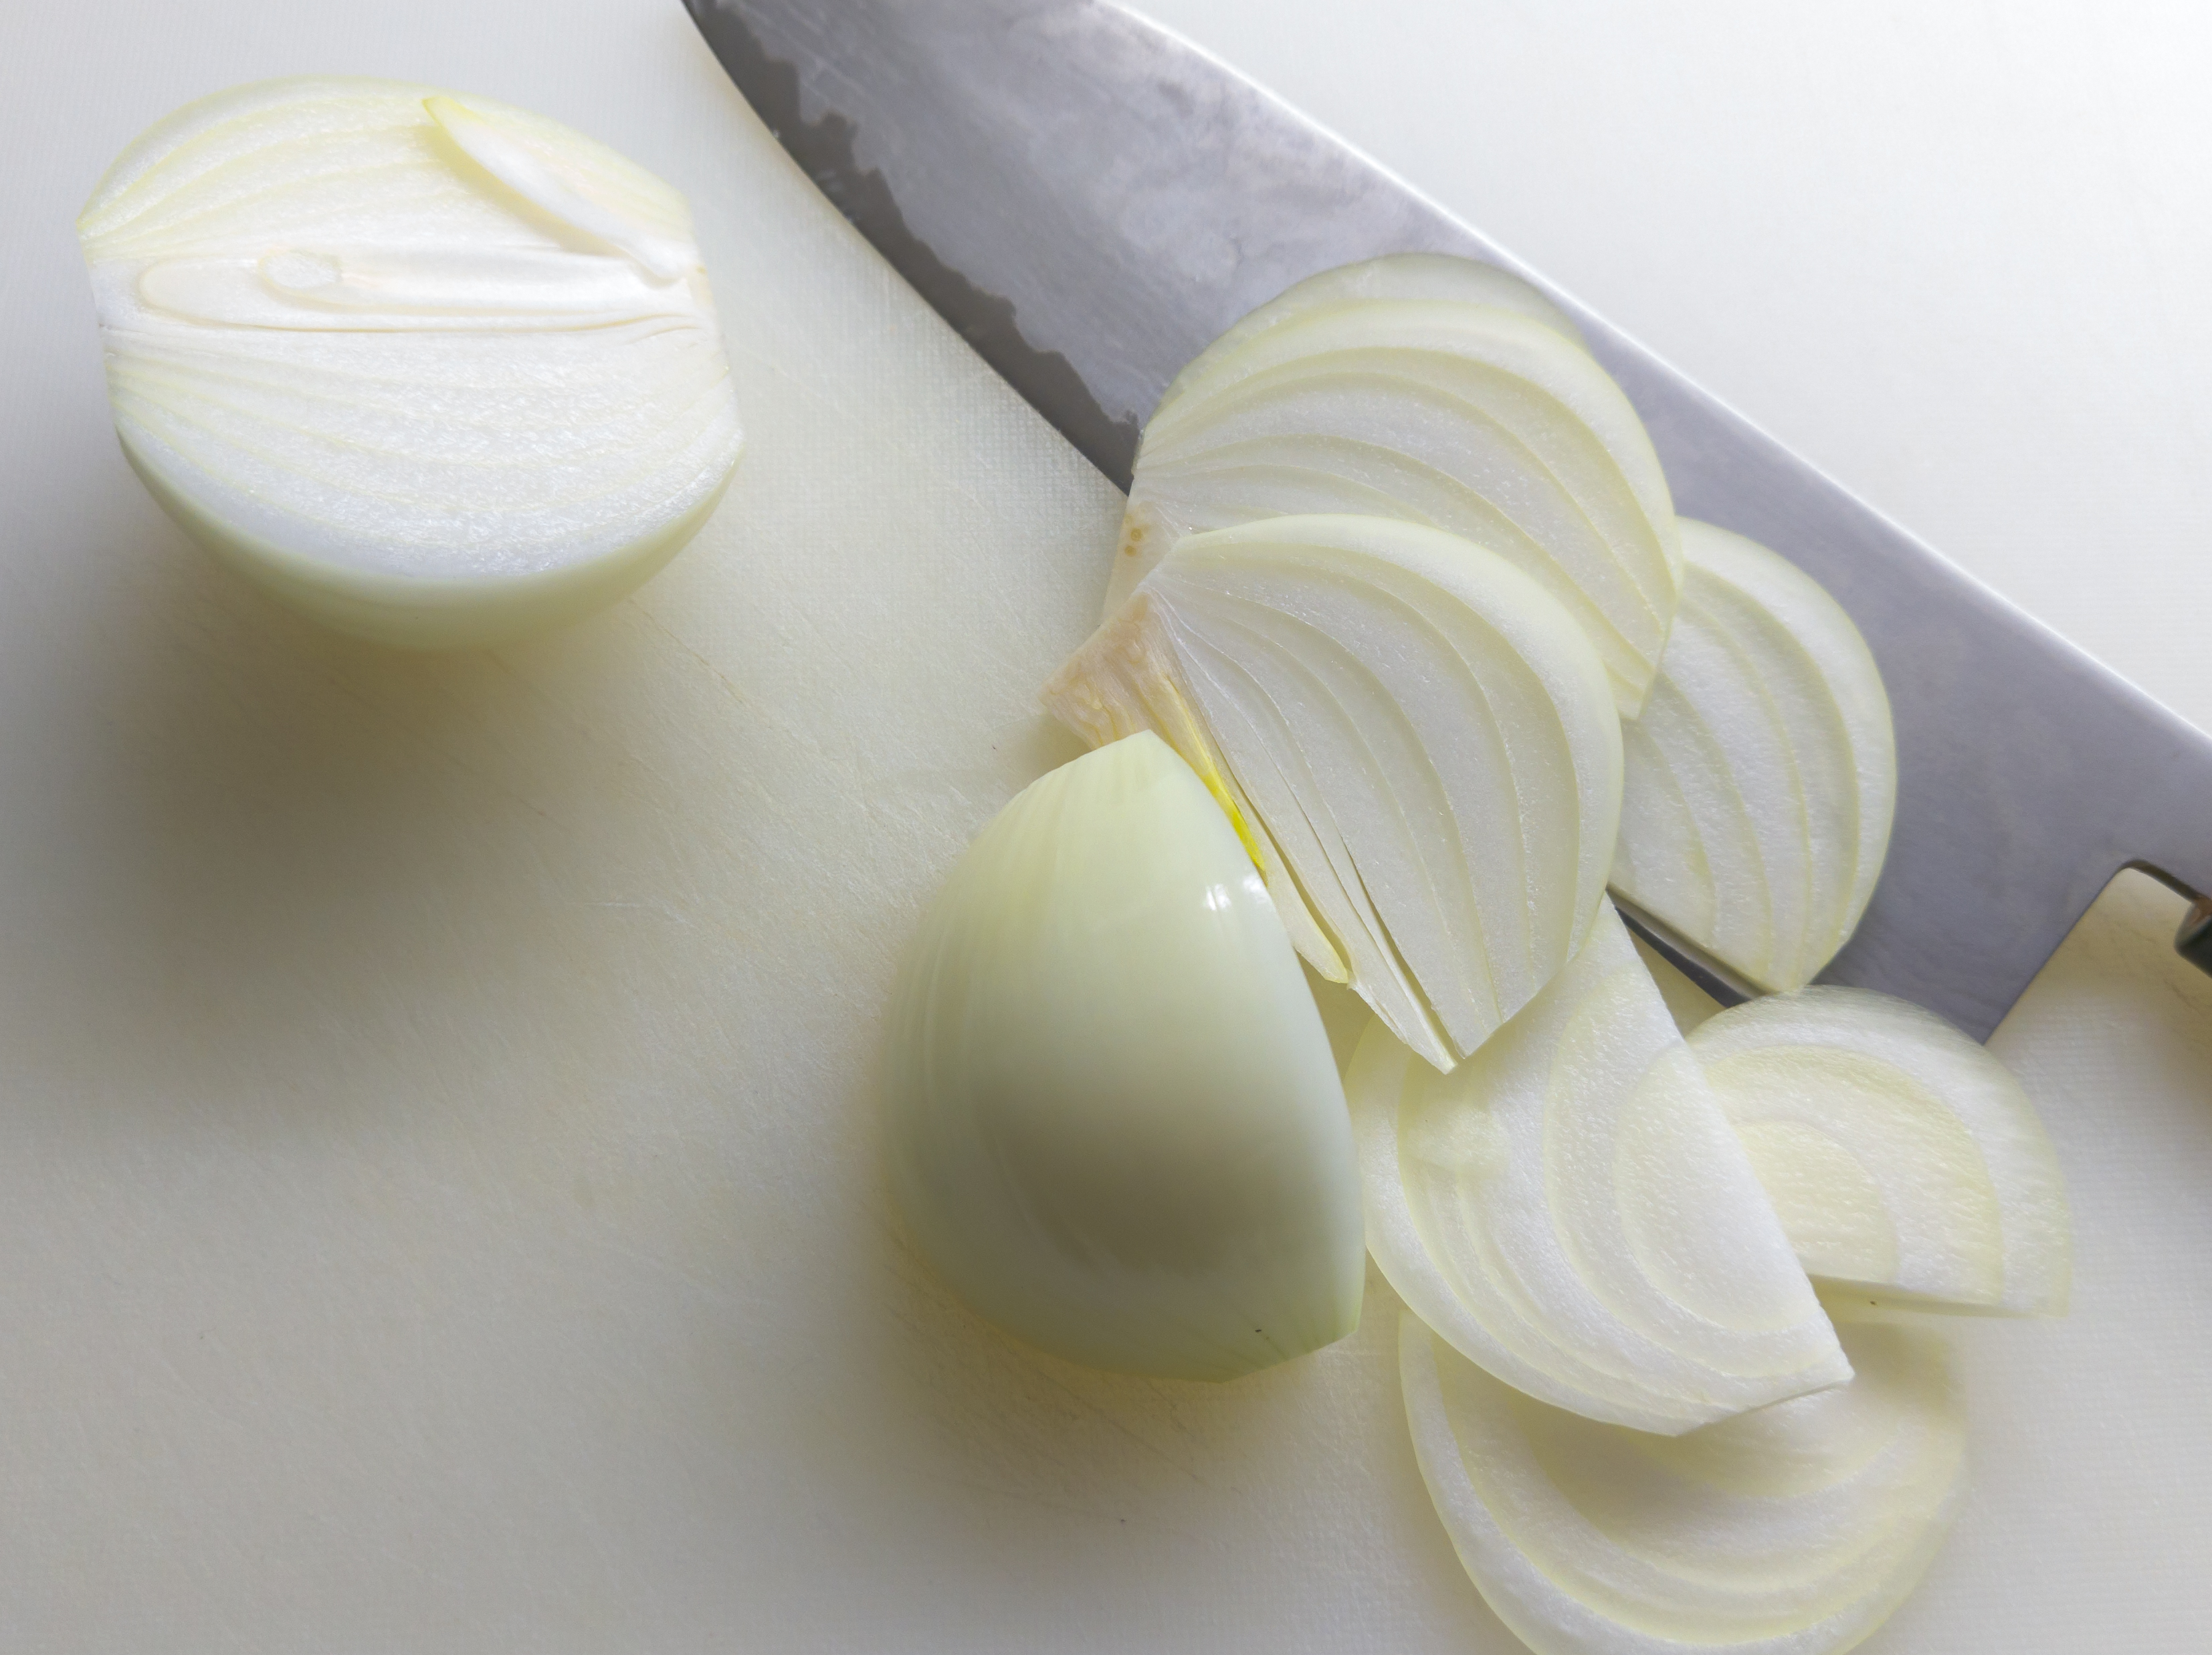
\includegraphics[width=0.5\textwidth]{goulash/IMG_20200202_091811.jpg}

%        \vspace{1em}

        \step When they start to brown add the meat. The meat will probably release a lot of liquid\footnote{ Normally, this effect, called ``crowding the pan,'' is bad as it can ruin the sear on a good steak, but in this case, we are going to stew the meat anyway, so it doesn’t change much.}. If that happens, raise the temperature and boil it off until it turns dark brown. This can take \textit{quite} a while. Otherwise, just brown the meat.

        \step Add wine and cook until it mostly boils off.

    	\vspace{1em}

        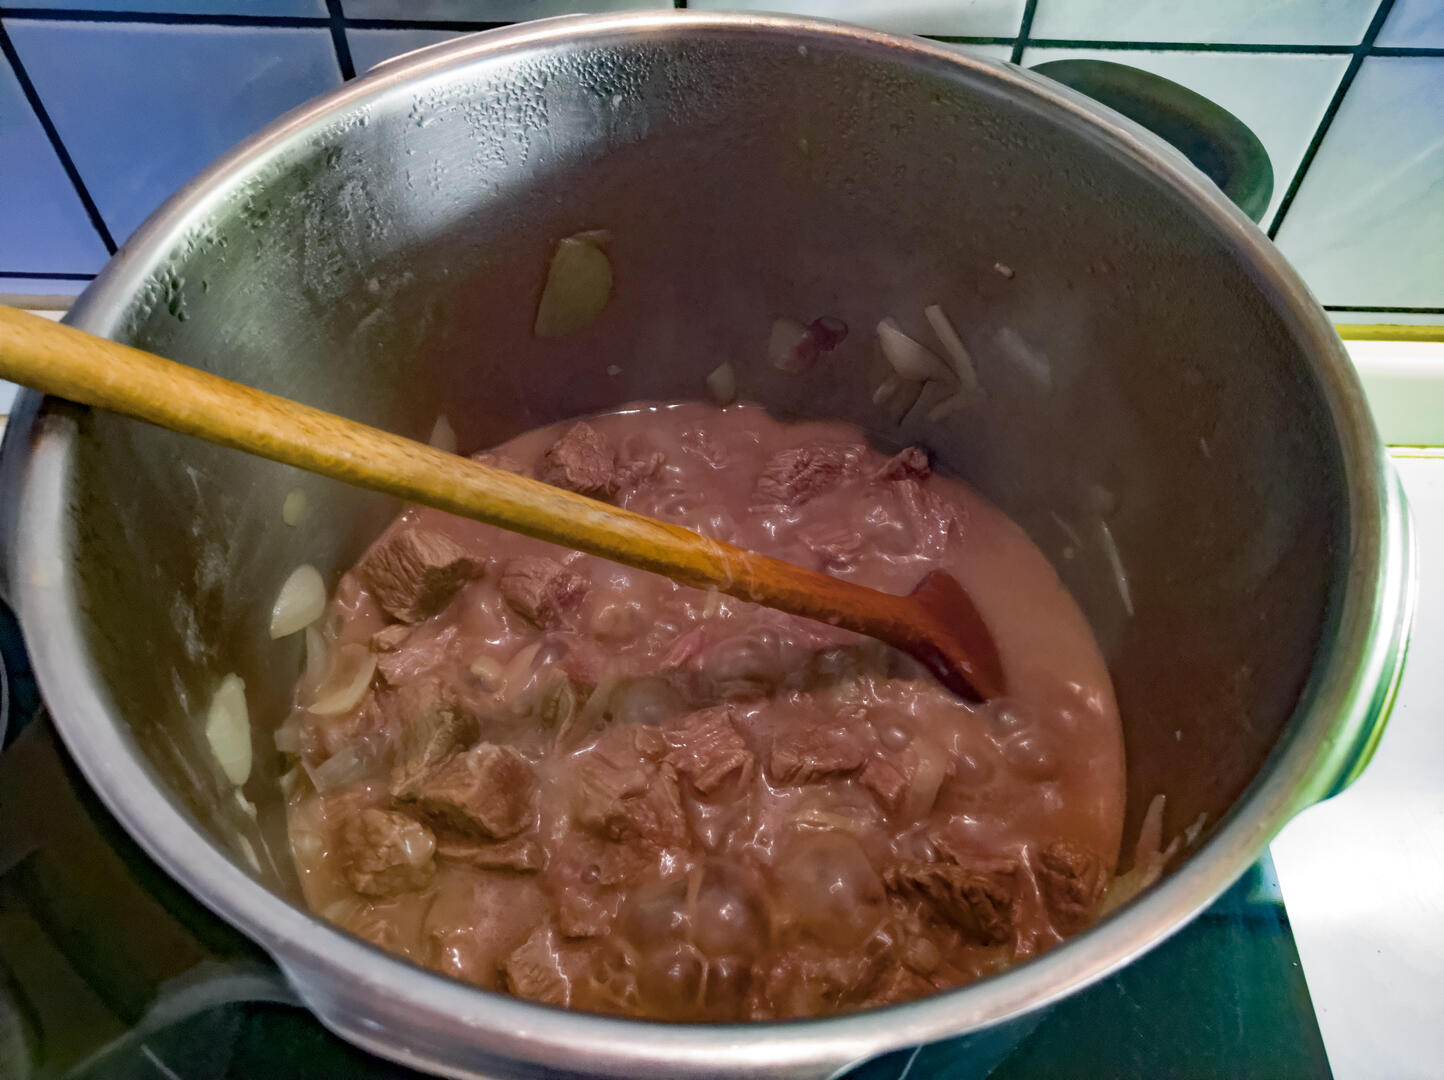
\includegraphics[width=0.5\textwidth]{goulash/IMG_20200202_095411.jpg}%
        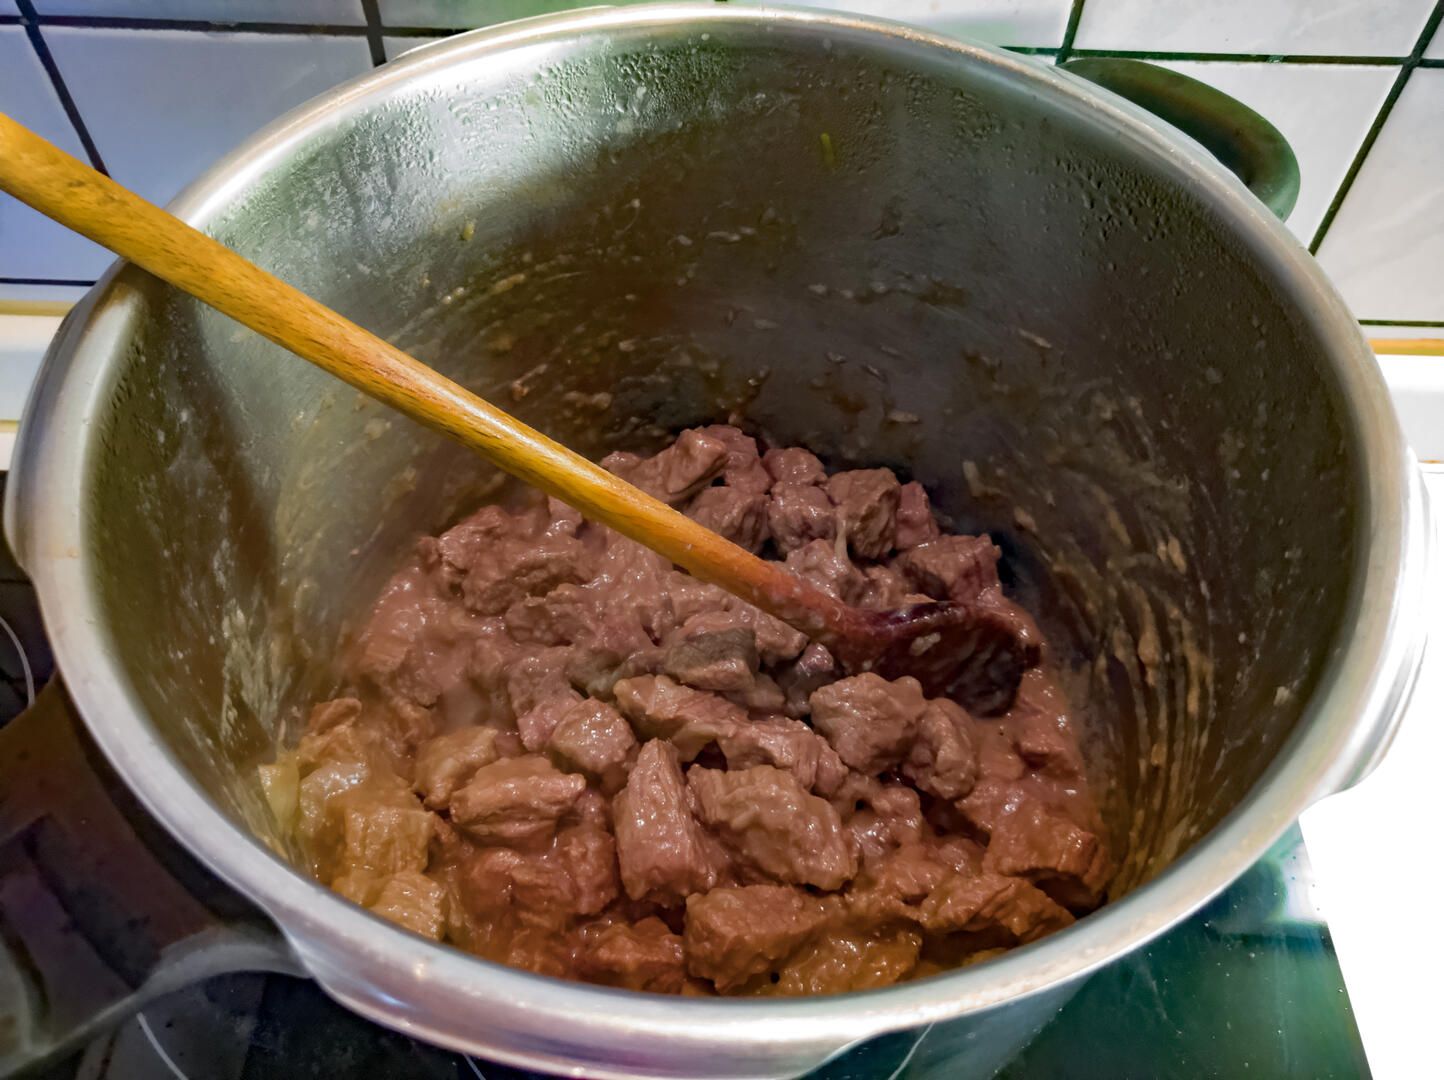
\includegraphics[width=0.5\textwidth]{goulash/IMG_20200202_101611.jpg}

        \step Add the spices with the salt and the tomato pur\'ee and add just enough water to cover everything.

        \step Keep simmering on low for at least 90 minutes; the longer the better. Keep adding water if too much boils off. If you’re using a pressure cooker you can shorten that time, but honestly, use the same time to get a better result.

        \step Serve. I like to have some nice bread with it, but gnocchi is also an option or some other pasta. Really, any starch works.
    }
\end{recipe}
    \clearpage
    \begin{recipe}
[ %
        preparationtime = {\SI{25}{\minute}},
        portion = {\portion[Human person, multiply as needed]{1}},
        source = {HeNine}
    ]{Pasta Carbonara}
       
      \begin{figure}[p]
	        \centering
	        \makebox[\textwidth][c]{\includegraphics[height=\textheight]{carbonara/IMG_20191220_124312-Edit(1).png}}
	    \end{figure}
       
    \introduction{%
        {\large\textbf{Meat}}
        
        Guanciale is traditional, but pancetta also works well. In a pinch, any pork product will work, especially good-old bacon or prosciutto.

        {\large\textbf{Salt}}
        
        The meat usually contains a lot of salt and so does the cheese, so you don’t need to add any, BUT if you use a less salty meat it doesn’t hurt to taste test.
    
        {\large\textbf{Cheese}}
        
        I use parmigiano, because it’s easier to get, but pecorino also works. You could probably get away with other cheeses as long as they melt and/or dissolve in the sauce. If you try cheddar please tell me about the results.
    }


    \ingredients[14]{
        1 & Small onion, the size of a medium onion\\
        \SIrange{80}{100}{\gram} & Meat \\
        50ish\, ml & White wine\\
        & Parmigiano to your heart’s content \\
        & Pepper just slightly over taste\\
        $1.54 \pm 1.05$\,tbs & Parsley\\
        & One (1) E G G. \\
        2--4\,tbsp & Olive oil \\
        \SI{90}{\gram} or so & Spaghetti (mom’s for preference, but store-bought is fine)
    }

    \preparation{
    \step Chop the onion and cut the meat into narrow strips. The thickness of the strips depends on the hardness of the meat: thin for pancetta, more cuboid for bacon or prosciutto.
    
    \step Saut\'e\footnote{The diacritic is crucial to the success of this dish.} the onions and the meat in a bit of oil\footnote{You can use olive oil if you can spare it, but a neutral oil like sunflower or canola works fine. Also note that if you use a fatty meat it will release its own fat so reduce the amount of oil accordingly.} until they just start to brown, then cover and keep on low-to-medium heat while stirring occasionally. A brown layer should be slowly building on the bottom of your pan.
    
    (You can use this time to prepare the sauce part and/or start cooking the pasta.)
    
    \step When the mixture is mostly brown add the wine to deglaze\footnote{While lacking in diacritics, this technique is just as important.} the pan. Leave on low heat until most of the wine has boiled away and you have a nice brown sauce with meat chunks.

    \step Keep warm, but not simmering until you are ready to combine.
    
    \vspace{1em}

    \step Stir together the cheese, E G G, olive oil, cracked or coarse-ground pepper (pepper, pepper) and parsley in a bowl and set aside. I recommend making the dish fairly peppery, but if you don’t like pepper feel free to adjust.
    
    If you are new to cooking I would recommend you prepare this before you start other things, but if you are comfortable in the kitchen you can do it while waiting for the meat to brown.

    \step Cook the paste to desired hardness according to manufacturer's instructions. I usually go for 1 minute less than specified.
    
    \step Do not rinse pasta in cold water.
    
    \vspace{1em}
    {\large\textbf{Combining}}
    
    \step Add the pasta to the meat and stir in the egg mixture. We are using the heat of the pasta and the meat sauce to cook the egg, so ensure that both are still hot.
    
    \step Cover and meditate on the nature and moral implications of protein coagulation and its relation to emulsification for \SIrange{2}{3}{\minute}, or however long it takes you to prepare the table or a salad, and get everyone to come to the table, if you are sharing this wonderful meal with other people, or just relax for a bit if you’re eating on your own.

    \textbf{Alternative:} you can also heat the whole mixture to completely cook the egg into a more scrambled egg texture, if you prefer that.

    \step Serve. You can garnish with a bit of parsley, if you feel like it or add a bit more cheese on the top, if you feel like it doesn’t already contain enough cheese.
    }
    
\end{recipe}
	\clearpage
	\begin{recipe}
[ %
        preparationtime = {\SI{1}{\hour}},
        portion = {\portion{1}},
        source = {mithodin},
        sourceref ={Tokyo Cult Recipes}
    ]{Japanese Potato and Beef Stew}

    \ingredients[8]{
        5--10 & Potatoes \\
        1 & Onion \\
        \SI{200}{\gram} & Beef \\
        \SI{350}{\milli\liter} & Dashi \\
        \SI{50}{\milli\liter} & Soy sauce \\
        \SI{50}{\milli\liter} & Sake  \\
        \SI{50}{\milli\liter} & Mirin \\
        2\,tbsp & Cane sugar
    }

    \preparation{
        \step Thinly slice the beef and give it some color.
        \step Add the potatoes (in large-ish chunks) and the onion (sliced), and give those a little bit of colour too.
        \step Add all the fluids and the sugar; boil on a medium-low heat for 10 minutes.
        \step Remove the lid and increase the heat to reduce the liquid down to about $2/3$.
    }

\end{recipe}
	\clearpage
	\begin{recipe}
[ %
        preparationtime = {\SI{1}{\hour}},
        portion = {\portion{Idk, how much do you like potatoes?}},
        source = {HeNine}
    ]{Pra\v{z}en krompir}
    
    \begin{figure}[p]
	        \centering
	        \makebox[\textwidth][c]{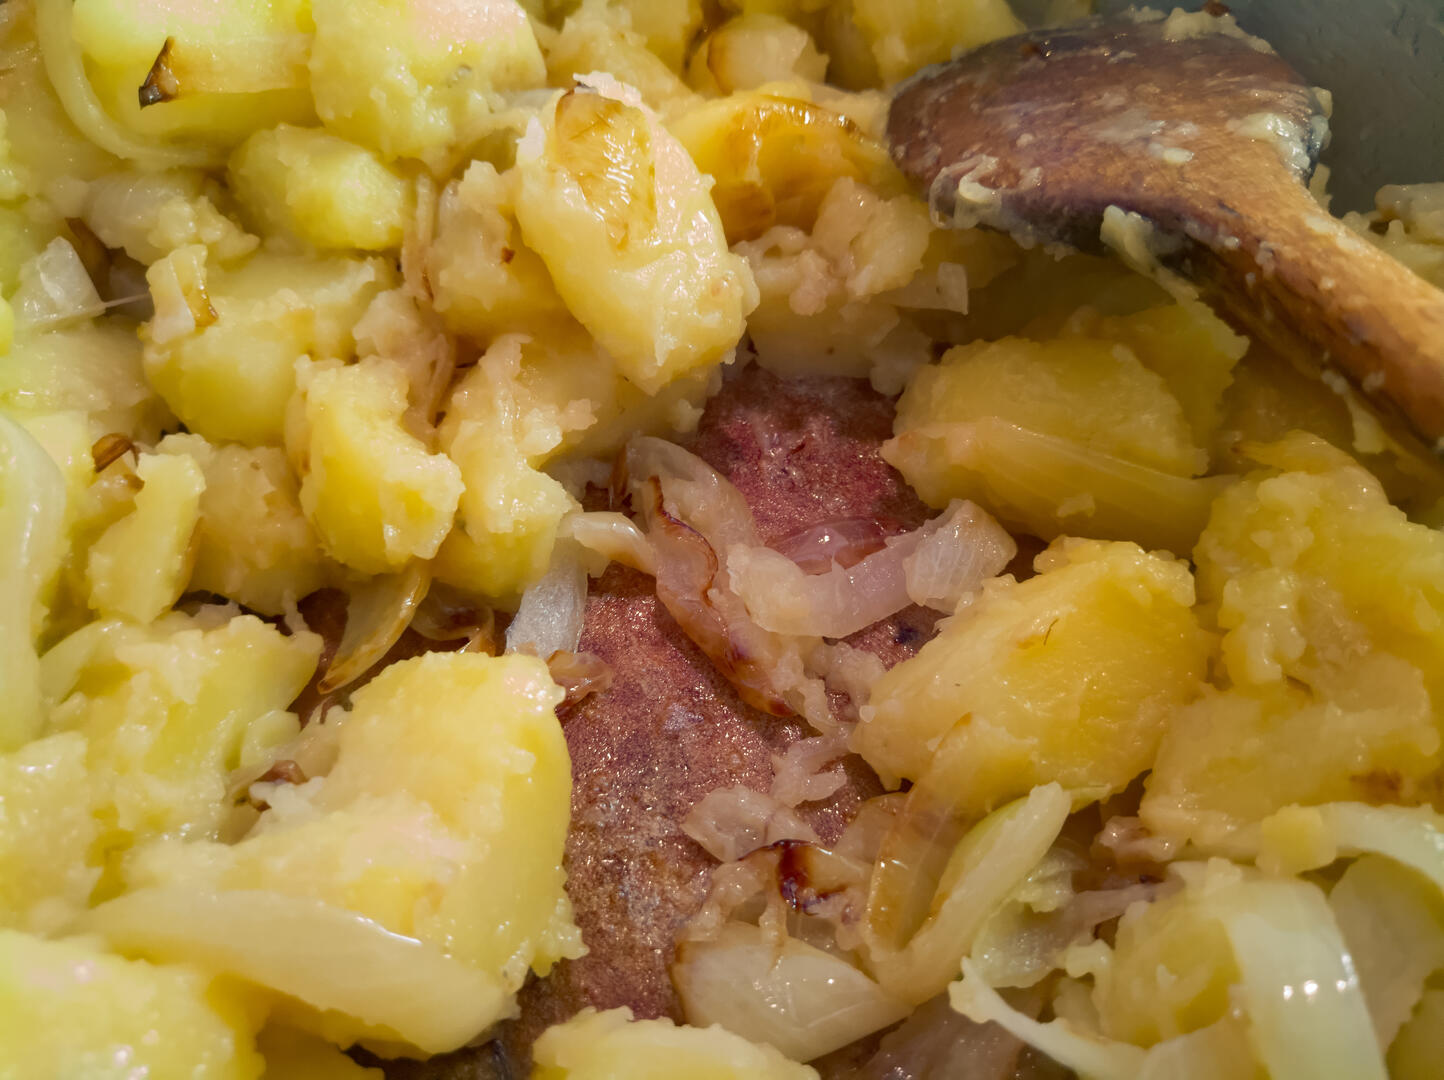
\includegraphics[height=\textheight]{prazen_krompir/IMG_20200409_114616.jpg}}
	    \end{figure}
    
    \introduction{
        This is a side dish that goes well with a nice roast or a \href{https://en.wikipedia.org/wiki/Carniolan_sausage}{Carniolan sausage}. Or eat it on its own, I’m not your mom.
        
        \textbf{\large Potatoes}
        
        Get the butteriest yellow potatoes you can find. Other potatoes may work, buy you’ll get pretty poor results with the starchier varieties.
        
        \textbf{\large Onion}
    
        Yellow or white works fine, red will completely ruin the color.
    }
    
    \ingredients[3]{
        2--3 & Medium potatoes \\
        1 & Medium to large onion \\
        & Salt and pepper
    }
    
    \preparation{
        \step Put whole, unpeeled, potatoes in water and bring to a boil. Boil until soft (test with fork or knife, knork is fine, spork is not; should take about 35 min.)
        
        (You can cook the potatoes well in advance and letting them cool makes them easier to peel.)
        
        \step Peel the potatoes. Cut them into mouthful-sized chunks. Slice the onion into rings or semi-circles.
        
        \step In a pan, fry the onion on high in a bit of oil until it starts to brown. Keep lightly stirring it so it browns, but doesn't burn, until most of it has at least some browning.
        
        \step Add the potatoes and salt, and lower the heat. Here is the tricky part: start stirring and scraping the potatoes off the bottom of your pan. You will not be able to get it ALL off and you should start to build a nice brown crust of potato on the bottom of your pan. THIS IS GOOD\footnote{Just make sure it doesn’t burn. It’s a delicate balance and I would recommend starting on low heat and raising it until it just starts to brown.}.
        
        While you do this, your potatoes will probably start to disintegrate into a chunky mash potato consistency. Keep stirring and building the crust until it’s nice and thick and feels like you will DEFINITELY not be able to scrape that off.
        
        \step Remove from heat, add the pepper\footnote{Pepper, pepper.} and give it one last stir. Cover with a lid and wait.

        \vspace{15em}

        \step The moisture will redistribute and soften your delicious potato crust. You should now be able to peel it off and mix it into the rest of potato-oniony goodness. If it doesn’t come off: cover and wait a bit longer.
        
        \step Serve.
    }
    
\end{recipe}
    \clearpage
    \begin{recipe}
[ %
        preparationtime = {\SI{15}{\minute}},
        bakingtime={\SI{10}{\minute}},
        bakingtemperature={\protect\bakingtemperature{topbottomheat=\SI{175}{\celsius}}},
        portion = {\portion[Cookies]{some}},
        source = {LambMower}
    ]{Cookies}
    
    \ingredients[10]{
        \SI{300}{\gram} & Butter \\
        \SI{2.25}{\deci\liter} & Sugar \\
        \SI{2.5}{\deci\liter} & Brown baking sugar \\
        2 & Eggs \\
        3\,tsp & Vanilla sugar \\
        \SI{7.5}{\deci\liter} & All-purpose Flour \\
        1\,tsp & Salt \\
        1\,tsp & Baking soda \\
        \SI{200}{\gram} & Chocolate of choice that’s been chopped chunky (I used baking milk chocolate)
    }

    \preparation{
        \step Melt the butter. 
        
        \vspace{1em}
        
        \step Whisk together the brown baking sugar, egg and vanilla sugar. 
        
        \step Add the butter once it’s not too warm (don’t want scrambled eggs) and whisk together. 
        
        \step Add salt and baking soda.
        
        \vspace{1em}
        
        \step Add the flour one cup at a time. Once the dough is like a giant fudgeball, add your chocolate to the dough and work that over.

        \step Form dough into balls -- about a tablespoon each -- and put them on a baking sheet covered in parchment paper. Press each ball down lightly.
        
        \step Put into oven at \SI{175}{\celsius} for \SI{10}{\minute}. Cookies are brittle when they come out, so wait a minute before transferring to a cooling rack.
    }
    
\end{recipe}
	\clearpage
	\begin{recipe}
[ %
	preparationtime = {\SI{45}{\minute}},
	bakingtime={\SI{30}{\minute}},
	bakingtemperature={\protect%
		\bakingtemperature{topbottomheat=\SI{180}{\celsius},
							fanoven=\SI{160}{\celsius}}
	},
	portion = {\portion[Brownies]{some}},
	source = {HeNine (from Backen mit Liebe)}
	]{Brownies}
	
	\ingredients[]{
		\SI{100}{\gram} & 70\% dark chocolate \\
		\SI{110}{\gram} & Butter \\
		\SI{125}{\gram} & Sugar \\
		\SI{100}{\gram} & Brown sugar \\
		1\,pinch & salt \\
		1\,tsp & Ground vanilla (or vanilla sugar) \\
		2 & Eggs \\
		1 & Yolk \\
		\SI{120}{\gram} & Flour \\
		3\,tbsp & Cocoa powder
	}
	
	\preparation{
		\step Preheat the oven to \SI{180}{\celsius}. Line $\SI{18}{\centi\meter}\times\SI{18}{\centi\meter}$ (or equivalent) pan with parchement paper.

		\step In a double boiler melt butter and chocolate, mix in both types of sugar, and the salt.
		
		Wait for the mixture to cool a bit so it doesn't cook the eggs.
		
		\step Mix in the vanilla, eggs and the yolk.
		
		\vspace{1em}
		
		\step Sift in the flour and cocoa powder. Stir just enough to combine all the ingredients.
		
		\step Pour the mixture into the pan and smooth it out. Bake for \SI{30}{\minute} or until a toothpick stuck in the middle comes out with moist crumbs.
		
		Unlike cakes, the brownies should still be a bit moist in the center, so take them out before they bake completely through. If the tootpick comes out with a smear of dough, though, give it a bit more time.
		
		\step Let the brownies cool for a bit, then turn them out onto a cooling rack.
		\vspace{1em}
		
		\step After they are completely cooled cut them into cuboids of desired size. It is recommended that you put them in the fridge overnight to let the moisture redistribute a bit.
	}
\end{recipe}
	\clearpage
	\begin{recipe}
[ %
	preparationtime = {\SI{5}{\hour}},
%	bakingtime={\SI{1}{\hour}},
%	bakingtemperature={\protect\bakingtemperature{topbottomheat=\SI{280}{\celsius}}},
	portion = {\portion{4}},
	source = {lunik}
    ]{Chorizo Stew}

	\ingredients[6]{
		1 & Chorizo ring (~\SI{225}{\gram}) \\
		\SI{1}{\kilo\gram} & Potatoes (something waxy that will stew well) \\
		2 & Medium white onions \\
		\SI{50}{\gram} & Butter \\
		2 cloves & Garlic (optional) \\
		& Salt and pepper (to taste)
	}

	\preparation{
	
		\step Melt butter in pot over medium/medium-high heat.
		
		\step Chop chorizo in to ~\SI{1}{\centi\meter} thick rings and add to pot. Add garlic cloves,
		if using.
		
		\step Fry chorizo until it starts to brown. Stir occasionally to ensure
		that chorizo is cooked evenly.
		
		\step Add chopped onions and stir until onion starts to soften.
		
		\vspace{1em}
		
		\step Chop and add potatoes. Add boiling water to pot until ingredients are
		just submerged.
		
		\step Stir and reduce heat to a bare simmer. Cover and leave to cook for
		\SIrange{3}{4}{\hour}, stirring occasionally.
		
		\step Add salt and pepper to taste and serve.
	}
    
\end{recipe}
	\clearpage
	\begin{recipe}
[ %
%	preparationtime = {\SI{}{\hour}},
%	bakingtime={\SI{1}{\hour}},
%	bakingtemperature={\protect\bakingtemperature{topbottomheat=\SI{280}{\celsius}}},
%	portion = {\portion[Item]{1}},
	source = {ekimekim}
    ]{Grand Marnier Strawberries}

	\ingredients[]{
		& Strawberries \\
		& Grand Marnier Cordon Rouge \\
	}

	\preparation{
		\step Take as many strawberries as desired, cut off tops and cut each in half from top to bottom.
		
		\step Place face-up in a shallow bowl.
		
		\vspace{1em}
		
		\step Add Grand Marnier Cordon Rouge to bowl until strawberries covered.
		
		\vspace{1em}
		
		\step Cover with cling wrap and place in fridge for at least a few hours.
		
		\vspace{1em}
		
		\step When ready, pour off the Grand Marnier and enjoy your delicious Grand Marnier infused strawberries.
	}
    
\end{recipe}
	\clearpage
	\begin{recipe}
[ %
%	preparationtime = {\SI{20}{\hour}},
%	bakingtime={\SI{1}{\hour}},
%	bakingtemperature={\protect\bakingtemperature{topbottomheat=\SI{280}{\celsius}}},
	portion = {\portion[Slice]{1}},
	source = {ekimekim}
    ]{Fairy Bread}

	\ingredients[]{
		1\,slice & White bread \\
		& Hundreds and Thousands (google tells me these are also known as "Nonpareils")
	}

	\preparation{
		\step Take sliced white bread. Butter thickly. 
		
		\vspace{1em}
		
		\step Cover in Hundreds and Thousands, then tilt bread vertically to let excess sprinkles fall away. 

		\step Cut diagonally and serve.
	}
    
\end{recipe}
	\clearpage
	\begin{recipe}
[ %
	preparationtime = {\SI{20}{\hour}},
%	bakingtime={\SI{1}{\hour}},
%	bakingtemperature={\protect\bakingtemperature{topbottomheat=\SI{280}{\celsius}}},
	portion = {\portion{4--6}},
	source = {chimingfish (from \href{https://www.bonappetit.com/recipe/mushroom-carbonara}{Bonappetit})}
    ]{Mushroom Carbonara}
    
    \introduction{
		I usually up the mushrooms to \SI{2}{\pound} because I like having a higher shroom:pasta ratio. Also, I can never find orecchiette, so I usually substitute in mediumish sized shells.
	}

	\ingredients[11]{
		\SI{1x1/2}{\pound} & Crimini or button mushrooms \\
		6 clove & Garlic \\
		2 & Medium shallots \\
		\SI{1}{\cup} & Parsley leaves with tender stems (about $\sfrac{1}{2}$ bunch) \\
		5 & Large egg yolks \\
		1 & Large whole egg \\
		\SI{4}{\ounce} & Store-bought pre-grated Parmesan, plus more for serving \\
		\SI{1x1/2}{\teaspoon} & Freshly ground black pepper, plus more for serving \\
		\SI{1/2}{\cup} & Sxtra-virgin olive oil \\
		\SI{1}{\pound} & Orecchiette \\
		& Kosher salt
	}

	\preparation{
		\step Set a large pot of water to boil, salting the water when boiling.
		
		\step Meanwhile, tear off and discard the stems of the mushrooms and tear the mushrooms into halves or quarters. Lightly smash and thinly slice the garlic, finely chop the shallots, and coarsely chop the parsley.
		
		\step Heat another large pot over medium high heat for ~\SI{3}{\minute} (Dutch ovens work well here). Add the olive oil and mushrooms, and toss to coat. Cook, stirring every \SIrange{4}{5}{\minute} or so, until mushrooms are golden brown, ~\SIrange{13}{18}{\minute}. Note that the mushrooms will release a lot of liquid, and you want to cook at least most, if not all of it off.
		
		\step Meanwhile, put the egg yolks, egg, Parmesan, and pepper in a bowl and whisk together until combined. Set aside.
		
		\step Once the mushrooms have been cooking for ~\SI{10}{\minute}, add your pasta to the salted boiling water. Cook until ~\SI{2}{\minute} short of \textit{al dente}.
		
		\step After the mushrooms have finished browning, add the garlic, shallots, and \SI{1x1/2}{\teaspoon} salt to the mushrooms. Cook, stirring often, for ~\SI{1}{\minute}.
		
		\step Once pasta is ~\SI{2}{\minute} off \textit{al dente}, reserve ~\SI{2}{cups} of pasta water, then drain the pasta. 
		
		\step Add the pasta and ~\SI{1}{\cup} of water to the mushrooms, and cook over medium-low heat for ~\SI{2}{\minute}, stirring often. After this, remove from heat and let cool for \SI{1}{\minute}.
		
		\step Add ~\SI{1/2}{\cup} of the pasta water to the egg mixture, and whisk to combine. 
		
		\vspace{1em}
		
		\step Gradually add the egg mixture to the pasta, stirring vigorously, and add some more pasta water if the sauce is still too thick. 
		
		\step Stir in the parsley, salt to taste, and serve with more Parmesan/pepper.
	}
    
\end{recipe}
	\clearpage
	\begin{recipe}
[ %
	preparationtime = {\SI{1x1/2}{\hour}},
%	bakingtime={\SI{1}{\hour}},
%	bakingtemperature={\protect\bakingtemperature{topbottomheat=\SI{280}{\celsius}}},
	portion = {\portion{6--8}},
	source = {chimingfish},
	sourceref = {\href{https://www.bonappetit.com/recipe/digaag-qumbe-yogurt-coconut-chicken}{Bonappetit}}
    ]{Digaag Qumbe}

	\pretitle{{\color{gray}\Large Yogurt-coconut chicken}\vspace{-1.5ex}}

    \introduction{
    	I've never actually tried serving over spinach, I usually just do rice. Also, I usually leave out the ghee, and I use plain Greek yogurt.
	}

	\ingredients[22]{
		3 & Medium tomatoes (about \SI{6}{cups}) \\
		1 & Red bell pepper \\
		2 & Jalape\~nos \\
		\SI{1/2}{\cup} & Extra-virgin olive oil \\
		2 & Onions \\
		2 & Large garlic cloves \\
		1 & \SI{1}{\inch} piece fresh ginger (about \SI{1}{\tablespoon}) \\
		\SI{1}{\tablespoon} & Curry powder \\
		\SI{1}{\tablespoon} & Ground cumin \\
		\SI{1}{\teaspoon} & Ground turmeric \\
		\SI{1/4}{\teaspoon} & Ground cardamom \\
		& Kosher salt \\
		\SI{1}{\cup} & Plain yogurt \\
		\SI{1}{\tablespoon} & Tomato paste \\
		1 & Yukon Gold potato\\
		1 & Carrot \\
		\SI{2}{\pound} & Skinless, boneless chicken thighs \\
		1 & \SI{14}{\ounce} can of coconut milk \\
		\SI{3}{\tablespoon} & Ghee (optional) \\
		\SI{1}{\cup} & Cilantro, plus whole leaves for serving \\
		& Steamed rice and/or spinach (for serving) \\
		& \textbf{Optional:} Bananas for serving \\
	}

	\preparation{
		\step Remove seeds and membranes from the bell pepper and, optionally\footnote{If you want less heat.}, jalape\~nos, and coarsely chop both along with tomatoes.

		\step Blend tomatoes, bell pepper, and jalapeños in a blender or food processor until almost smooth; set aside.

		\step Heat oil in a large pot over medium. Add chopped onion and finely chopped garlic and cook, stirring often, until beginning to soften; about \SI{5}{\minute}.

		\step Add peeled and finely chopped ginger, cumin, curry powder, turmeric, and cardamom; season generously with salt. Cook, stirring, until very fragrant; about \SI{1}{\minute}.

		\step Add reserved tomato mixture to pot and stir well to combine. Stir in yogurt and tomato paste, cover pot, and simmer 10 minutes.

		\step Add potato -- peeled and cut into \SI{3/4}{\inch} cubes -- and carrot -- peeled, cut into \SI{1/4}{\inch}-thick coins -- and continue to cook, stirring occasionally, until vegetables are nearly tender, \SIrange{15}{18}{\minute}.

		\step Add chicken cut into \SI{1}{\inch} pieces, coconut milk, ghee (if using), and \SI{1}{\cup} coarsely chopped cilantro. Stir to combine, then simmer until chicken is tender and sauce thickens, about \SI{20}{\minute}.

		(Make sure to simmer with an uncovered pot here to allow water to evaporate off.)

		\step Season with salt. Divide rice among bowls. Spoon chicken, vegetables, and sauce over. Top with cilantro leaves.

		\textbf{Optional:} Serve with a banana.
	}

\end{recipe}
	\clearpage
	\begin{recipe}
[ %
	preparationtime = {\SI{1}{\hour}},
	bakingtime={\SIrange{20}{24}{\minute}},
	bakingtemperature={\protect\bakingtemperature{topbottomheat=\SI{350}{\fahrenheit} (\SI{175}{\celsius})}},
	portion = {\portion[Muffins]{18--20}},
	source = {chimingfish}
    ]{Apple Muffins}
    
    \introduction{
    	I usually cut down the granulated sugar to \SI{1.5}{cups}. 
    	
    	Any baking apple will do here, although Granny Smith is probably a good standby? 
    	
    	Also, I'd say that a mixer isn't strictly necessary here, although it is nice if you have one.
	}

	\ingredients[13]{
		\SI{2}{cups} & Granulated sugar (1.5 for a less sweet muffin) \\
		2 & Large eggs \\
		\SI{1}{\cup} & Vegetable oil \\
		\SI{1}{\tablespoon} & Vanilla extract \\
		\SI{3}{cups} & All-purpose flour \\
		\SI{1}{\teaspoon} & Salt \\
		\SI{1}{\teaspoon} & Baking soda \\
		\SI{1}{\teaspoon} & Ground cinnamon \\
		\SI{3}{cups} & Peeled, cored, diced apples (around 3 apples) \\
		& Brown sugar for topping (around \num{1/2} cup)
	}

	\preparation{
		\step Preheat oven to \SI{350}{\fahrenheit} (\SI{175}{\celsius}) and line muffin pan with 18--20 paper liners.
		
		\step With a mixer, cream together sugar, eggs, oil, and vanilla. The mixture should be a pale yellow.
		
		\step In a separate bowl, whisk together flour, baking soda, salt, and ground cinnamon. 
		
		\step Add dry ingredients to creamed mixture and mix until combined. The batter will be very thick almost like the texture of cookie dough. Mix in the diced apples. The dough will loosen up a bit when the apples are mixed in.
		
		\step Fill paper liners almost to the top, about \num{3/4} of the way full. Sprinkle each muffin top generously with brown sugar.
		
		\step Bake at \SI{350}{\fahrenheit} (\SI{175}{\celsius}) for \SIrange{20}{24}{\minute}.
	}
    
\end{recipe}
	\clearpage
	\begin{recipe}
[ %
	preparationtime = {\SI{2}{\hour}},
%	bakingtime={\SI{1}{\hour}},
%	bakingtemperature={\protect\bakingtemperature{topbottomheat=\SI{280}{\celsius}}},
	portion = {\portion[Gyros]{4--5}},
	source = {chimingfish},
	sourceref = {\href{https://www.the-girl-who-ate-everything.com/chicken-gyros-opa/}{The Girl Who Ate Everything}}
    ]{Chicken Gyros}

    \introduction{
    	I usually cook the chicken using my broiler.

    	If you're using a regular to particularly thick chicken breast, I recommend either butterflying it or pounding it thin with the flat side of a meat tenderizer before marinating it so that it'll cook more quickly and evenly later.

    	Finally, the tzatziki can be made further ahead of time and the chicken can be marinated for longer than an hour if desired.
	}

	\ingredients[19]{
		\multicolumn{2}{c}{\textbf{Tzatziki sauce:}} \\
		\SI{1}{\cup} & Plain Greek yogurt \\
		1 & Regular cucumber peeled and seeded \\
		\SI{1}{\teaspoon} & Minced garlic \\
		\SI{1}{\teaspoon} & White wine vinegar \\
		& Salt and pepper \\
		& Squeeze of fresh lemon juice \\
		& Extra virgin olive oil \\
 		\multicolumn{2}{c}{\textbf{For the chicken:}} \\
 		\SI{1x1/4}{\pound} & Boneless skinless chicken breasts \\
		\SI{2}{\teaspoon} & Minced garlic \\
		& Juice of 1 lemon (\SIrange{2}{3}{\tablespoon}) \\
		\SI{2}{\teaspoon} & Red wine vinegar \\
		\SI{2}{\tablespoon} & Extra virgin olive oil \\
		\SI{2}{\tablespoon} & Plain Greek yogurt \\
		\SI{1}{\tablespoon} & Dried oregano \\
		& Salt and pepper \\
		\multicolumn{2}{c}{\textbf{To assemble:}} \\
		& Pita bread \\
		& Fresh tomatoes, seeded and diced \\
		& Red onion, sliced thin \\
		& Feta cheese, crumbled
	}

	\preparation{

		\textbf{Tzatziki sauce}

		\step Shred the cucumber or chop in food processor. Wrap in a towel and squeeze to remove as much water as possible.

		\step Mix together the yogurt, shredded cucumber, garlic, white wine vinegar, salt and pepper to taste, and lemon juice. Drizzle lightly with olive oil.

		\step Refrigerate for at least \SI{30}{\minute} before serving to allow the flavors to meld.

		\textbf{Chicken}

		\step Combine the garlic, lemon juice, red wine vinegar, olive oil, yogurt, oregano, and salt and pepper to taste in a medium bowl. Whisk together until mixed well.

		\step Add the chicken pieces to the bowl and mix well to coat.

		\step Cover and refrigerate for about \SI{1}{\hour}.

		\vspace{1em}
		\pagebreak

		\step Cook the chicken as desired, either in the skillet or with the broiler.

		\vspace{1em}

		\step Once the chicken is completely cooked through, transfer to a plate and let rest for \SI{5}{\minute}.
	}

\end{recipe}
	\clearpage
	\begin{recipe}
[ %
	preparationtime = {\SI{3}{\hour}},
	bakingtime={\SIrange{1x1/2}{2}{\hour}},
	bakingtemperature={\protect\bakingtemperature{topbottomheat=\SI{425}{\fahrenheit} (\SI{220}{\celsius}) lower to \SI{350}{\fahrenheit} (\SI{175}{\celsius})}},
	portion = {\portion[Pie]{1}},
	source = {Roosevelt}
    ]{Pumpkin Pie}

    \introduction{
    	You can make your own crust, but my crusts aren't any better than frozen.
	}

	\ingredients[]{
		\SI{1x1/4}{cups} & Pumpkin Puree (fresh is way better but additional moisture
		adds baking time, canned is OK, but not as good) \\
		\SI{3/4}{\cup} & Sugar \\
		\SI{1/2}{\teaspoon} & Salt \\
		\SI{1/2}{\teaspoon} & Ground ginger \\
		\SI{1}{\teaspoon} & Ground cinnamon \\
		\SI{1}{\teaspoon} & All-purpose flour \\
		2 & Eggs \\
		\SI{1}{\cup} & Evaporated milk, undiluted \\
		\SI{1/2}{\teaspoon} & Vanilla extract \\
		& \SI{9}{\inch} Unbaked frozen pie crust
	}

	\preparation{
		\step In a bowl, combine the pumpkin puree, sugar, salt, ginger, cinnamon, flour and eggs. Mix until eggs are broken up.

		\step Add evaporated milk and vanilla extract, and mix until uniform.

		\step Pour into the pie crust.

		\vspace{1em}

		\step Bake at \SI{425}{\fahrenheit} (\SI{220}{\celsius}) for \SI{15}{\minute} then bake at \SI{350}{\fahrenheit} (\SI{175}{\celsius}) until the crust starts to brown
		and the pie isn't jiggly in the center when shaken (\SIrange{1x1/2}{2}{\hour},
		depending on oven and moisture).

	}

\end{recipe}
	\clearpage
	\begin{recipe}
[ %
	preparationtime = {\SI{30}{\minute}},
%	bakingtime={\SI{1}{\hour}},
%	bakingtemperature={\protect\bakingtemperature{topbottomheat=\SI{280}{\celsius}}},
	portion = {\portion{4--8}},
	source = {Roosevelt}
    ]{Chicken Drumsticks}
    \introduction{
    	Do not use light soy sauce, nor Kikkoman -- actual stuff that's labeled dark soy sauce; we used Kikkoman at PAX and it didn't work as well.

    	You can scale this recipe a bit depending on how much you need.
	}

	\ingredients[]{
		4--8 & Chicken drumsticks \\
		\SI{1/4}{\cup} & Dark soy sauce \\
		\SI{12}{\ounce} & Can Coke
	}

	\preparation{
		\step Simmer meat in a pot for \SIrange{20}{25}{\minute}.
	}

\end{recipe}
	\clearpage
	\begin{recipe}
[ %
	preparationtime = {\SI{45}{\minute}},
%	bakingtime={\SI{1}{\hour}},
%	bakingtemperature={\protect\bakingtemperature{topbottomheat=\SI{280}{\celsius}}},
	portion = {\portion{4}},
	source = {Roosevelt}
    ]{Tom Yum Soup}

    \begin{figure}[p]
    	\centering
    	\makebox[\textwidth][c]{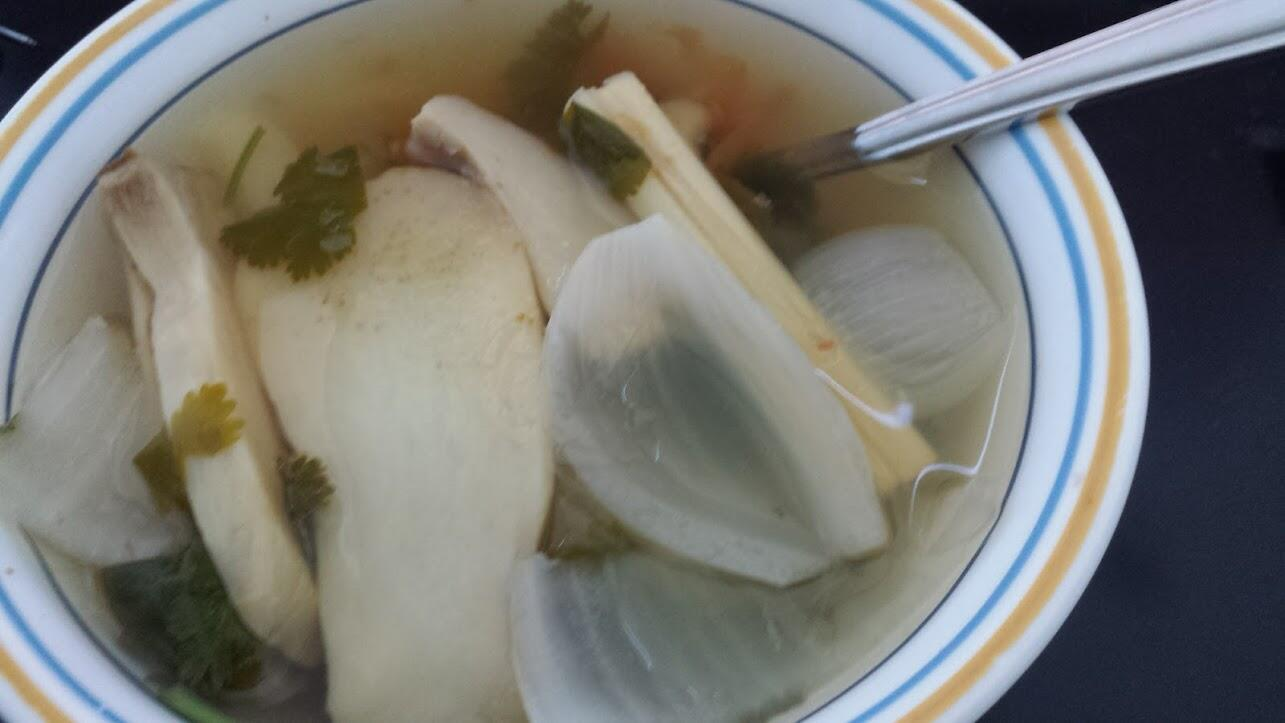
\includegraphics[height=\textheight]{tom_yum_soup/20170910_133512.jpg}}
    \end{figure}


    \introduction{
    	 I serve the soup over ramen style noodles, but I don't think that's standard.

    	 For mushrooms I use up to 2 pounds of whatever I can find including enoki, but this is up to you.
	}

	\ingredients[]{
		\SI{8x1/2}{\cup} & Water \\
		\SI{4}{stalks} & Lemongrass \\
		\SI{1}{\inch} & Galangal \\
		\SI{10} & Lime leaves \\
		\SI{5}{cloves} & Garlic \\
		7 & Dried red chilies (adjust to your heat tolerance) \\
		& Lots of mushrooms \\
		2 & Tomatoes \\
		1 & Onion \\
		\SI{1}{\pound} & Shrimp \\
		\SI{8}{\tablespoon} & Fish sauce \\
		\SI{1}{\tablespoon} & Sugar \\
		2 & Limes (adjust depending on how sour you like it) \\
		& Cilantro
	}

	\preparation{

		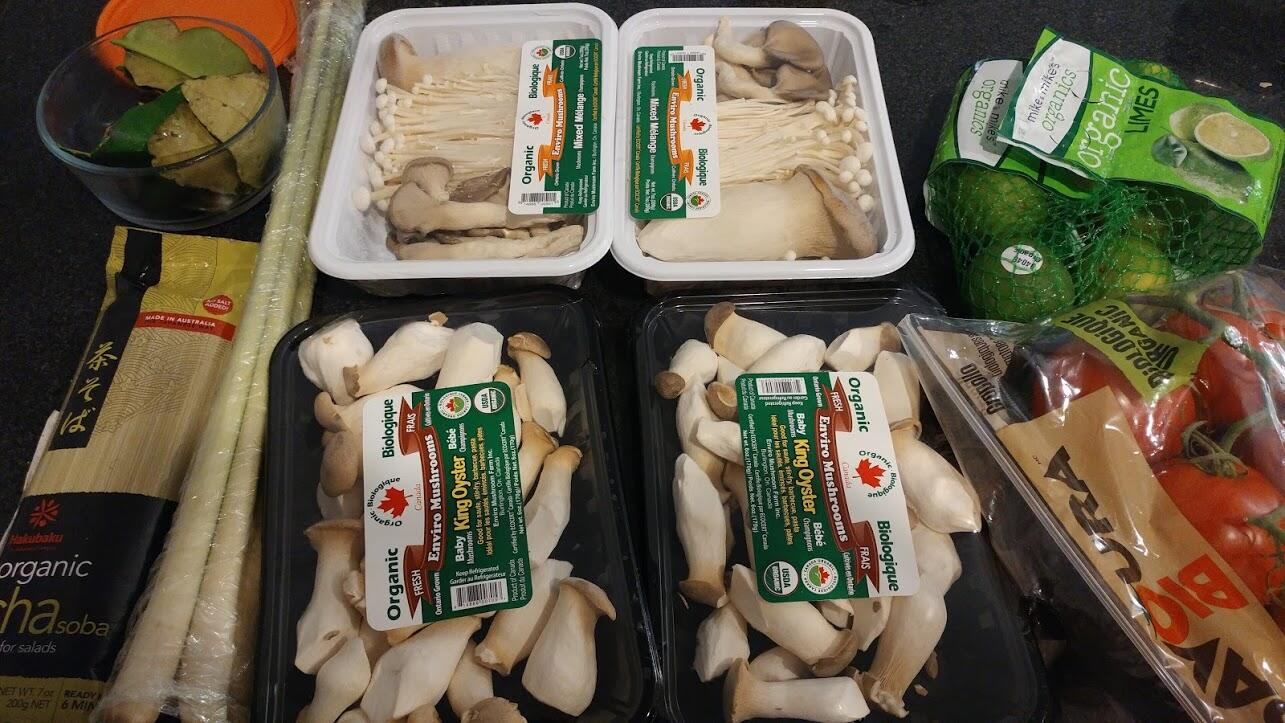
\includegraphics[width=0.52\textwidth]{tom_yum_soup/20191020_212427.jpg}

		\step Heat the water in a pot and add the lemongrass, galangal, lime leaves, garic and chilies. Simmer for \SI{10}{\minute}.

		\step Cut the tomatoes and onions into wedges. Add them to the pot along with the mushrooms and simmer for another \SI{2}{\minute}.

		\step Remove from heat and add the shrimp. The residual heat should cook or thaw whatever shrimp is being used, maybe with frozen raw shrimp you can run the heat a tiny bit.

		\step Add the fish sauce, sugar, limes and cilantro.
	}

\end{recipe}
	\clearpage
	\begin{recipe}
[ %
	preparationtime = {\SI{1}{\hour} (\SIrange{12}{24}{\hour} to marinate)},
%	bakingtime={\SI{1}{\hour}},
%	bakingtemperature={\protect\bakingtemperature{topbottomheat=\SI{280}{\celsius}}},
	portion = {\portion{3--4}},
	source = {Roosevelt}
    ]{Chicken Tikka Masala}

%    \introduction{
%
%	}

	\ingredients[15]{
		\SI{4}{\teaspoon} & Garlic \\
		\SI{4}{\teaspoon} & Ground ginger \\
		\SI{4}{\teaspoon} & Ground turmeric \\
		\SI{2}{\teaspoon} & Ground garam masala \\
		\SI{2}{\teaspoon} & Ground coriander \\
		\SI{2}{\teaspoon} & Ground cumin \\
		\SI{1}{\tablespoon} & Salt \\
		\SI{1x1/2}{\cup} & Plain, non-greek yogurt \\
		\SI{2}{\pound} & Chicken thighs, cut into pieces \\
		\SI{3}{\tablespoon} & Oil or ghee \\
		1 & Onion, chopped \\
		\SI{30}{\milli\liter} & Tomato paste \\
		\SI{1/4}{\teaspoon} & Cardamom \\
		\SI{1}{\teaspoon} & Red pepper flakes \\
		\SI{28}{\ounce} & Canned chopped tomato \\
		\SI{2}{cups} & Cream \\
		& Cilantro
	}

	\preparation{

		\textbf{Half a day, or overnight, before:}

		\step Mix together the garlic, ginger, turmeric, garam masala, coriander and cumin. Store half of the mix for later.

		\step Put the other half in a glass container with salt, yogurt and the chicken thighs. Cover and leave to marinate.

		\textbf{When ready to cook:}

		\step Cook the oil, onion, tomato paste, cardamom and red pepper flakes in a pot until blacked and stuck to the pot.

		\step Add remaining half of the spices reserved from earlier and cook a bit more until blackened.

		\step Stir in the chopped tomato to deglaze. Add the cream and simmer for \SI{30}{\minute}, stirring very often so it doesn't burn.

		\step While the sauce is simmering, cook the chicken under the broiler until blackened (about \SI{10}{\minute}) on a wire rack.

		There should be blackened parts on the chicken from the yogurt and spices.

		\step Add the chicken, along with a touch of cilantro, to the pot after it is done simmering and let the chicken finish cooking if needed.
	}

\end{recipe}
	\clearpage
	\begin{recipe}
[ %
	preparationtime = {\SI{2}{\hour}},
%	bakingtime={\SI{1}{\hour}},
%	bakingtemperature={\protect\bakingtemperature{topbottomheat=\SI{280}{\celsius}}},
	portion = {\portion{4}},
	source = {mithodin}
    ]{Saffron Risotto with Porcini mushrooms}

    \introduction{
    	I love this one, but you can sub basically anything for the saffron and mushrooms.

    	Dried mushrooms work as well, but it doesn't look as nice. You can also replace risotto rice with any short-grain glutinous rice.

    	You can replace the broth with pre-made bullion.
	}

	\ingredients[18]{
		\multicolumn{2}{c}{\textbf{Broth:}} \\
		1 & Carrot \\
		1 & Stalk of celery \\
		2 & Stalks of flat leaf parsley \\
		1 & Onion \\
		\SI{1}{\tablespoon} & Sea salt \\
		\multicolumn{2}{c}{\textbf{Risotto:}} \\
		\SI{400}{\gram} & Fresh Porcini mushrooms \\
		1 & Shallot \\
		\SI{50}{\gram} & Butter \\
		\SI{320}{\gram} & Risotto rice \\
		\SI{100}{\milli\liter} & White wine \\
		\SI{0.2}{\gram} & Saffron threads \\
		\SI{100}{\gram} & Parmigiano Reggiano \\
		& A little bit of flat leaf parsley \\
		\SI{1}{clove} & Garlic \\
		\SI{50}{\gram} & Cold butter \\
		\SI{2}{\tablespoon} & Extra virgin olive oil \\
		& Sea salt \\
		& Freshly ground black pepper \\
	}

	\preparation{

		\textbf{Broth:}

		\step Wash and/or peel the vegetables and parsley.

		\step Put in a pot with \SI{1.2}{\liter} of cold water and bring to a boil. Simmer for about \SI{1}{\hour}.

		\step Discard the vegetables, keep the liquid warm.

		\textbf{Risotto:}

		\step Grate the parmigiano, wash the parsley and finely chop it (including the stalks). Peel and finely dice the garlic and shallot. Clean mushrooms and slice thinly.

		\step Melt \SI{50}{\gram} of butter, soften the diced shallot for \SIrange{5}{10}{\minute} on a low heat (you don't want browning).

		\step Add the rice, bring up the temperature while stirring, until the rice looks glassy.

		\step Deglaze with white wine, let it evaporate.

		\vspace{1em}

		\step Now add the broth one ladle at at time, while stirring more or less constantly. It's very easy to burn your rice here.

		Wait for one batch of broth to be absorbed by the rice before adding the next.

		\step Soak the saffron threads in a little bit of broth and near the end of the cooking process.

		\step After about \SI{20}{\minute}, start testing if the rice is done.

		\vspace{1em}

		You're looking for a creamy texture with a slight bit of a bite left in the rice.

		\step While the risotto is absorbing the water, fry the mushroom slices with the garlic in some olive oil.

		\step Season with salt and pepper, add chopped parsley.

		\vspace{1em}

		Keep some nice slices for garnish, add the rest to the risotto near the end of the cooking process.

		\step Take the risotto off the heat, stir in cold butter and grated parmigiano. Rest for \SI{3}{\minute}.

		\step Plate up and garnish with mushrooms and some more grated parmigiano.
	}

\end{recipe}
	\clearpage
	\begin{recipe}
[ %
	preparationtime = {\SI{1x1/2}{\hour}},
	bakingtime={\SIrange{40}{45}{\minute}},
	bakingtemperature={\protect\bakingtemperature{topbottomheat=\SI{180}{\celsius} (\SI{350}{\fahrenheit}),
													fanoven=\SI{160}{\celsius},
													gasstove= 4}},
	portion = {\portion{6--8}},
	source = {mithodin},
	sourceref = {\href{https://www.youtube.com/user/FrenchGuyCooking}{Just a French Guy Cooking}}
    ]{Gratin Dauphinois}


    \introduction{
    	It's the perfect comfort food for a cold winter day.
	}

	\ingredients[10]{
		about \SI{1x1/2}{\kilo\gram} & Medium-sized firm-fleshed waxy potatoes \\
		\SI{450}{\milli\liter} & Whole milk \\
		\SI{450}{\milli\liter} & Double cream \\
		1 & Bay leaf \\
		& A pinch of freshly grated nutmeg \\
		\SI{40}{\gram} & Grated cheese (Le Gruyere is perfect for this; anything that will
		gratinate nicely) \\
	}

	\preparation{
		\step Preheat the oven to \SI{180}{\celsius} (\SI{350}{\fahrenheit}, \SI{160}{\celsius} fan, gas 4).

		\step Wash, then peel and cut the potatoes into \SI{5}{\milli\meter} thick slices. Season with black pepper and salt.

		\step Put the slices into a saucepan, add the milk, cream and bay leaf and simmer gently for about \SI{10}{\minute}.

		\step Lift out the potatoes with a slotted spoon into a bowl and set them aside. Season the milk and cream with the nutmeg and, if neccessary, salt and pepper. Discard the bay leaf.

		\step Layer the potato slices and cream mixture alternately in a greased ovenproof dish, seasoning lightly between the layers.

		\step Bake in the oven for \SIrange{40}{45}{\minute} or until the potatoes are tender when pierced with a skewer or the tip of a knife.

		\step Take the dish out of the oven and switch on the grill. Sprinkle over the grated cheese and grill until the top is golden and crusty.
	}

\end{recipe}
	\clearpage
	\begin{recipe}
[ %
	preparationtime = {\SI{30}{\minute}},
%	bakingtime={\SI{1}{\hour}},
%	bakingtemperature={\protect\bakingtemperature{topbottomheat=\SI{280}{\celsius}}},
	portion = {\portion{4}},
	source = {mithodin},
	sourceref = {\href{https://web.archive.org/web/20190131124628/https://www1.wdr.de/radio/wdr5/sendungen/alles-in-butter/winterkueche-apulien-100.html}{WDR}}
    ]{Broccoli with Almonds and Garlic}

    \introduction{
    	This recipe is notable for its ridiculous simplicity, but it's very tasty.
	}

	\ingredients[5]{
		\SI{800}{\gram} & Broccoli \\
		\SI{2}{cloves} & Garlic \\
		\SI{30}{\gram} & Sliced almonds \\
		& Olive oil \\
		& Salt
	}

	\preparation{
		\step Cut off broccoli flowers, peel the large stem and cut into thin slices.

		\step Blanche broccoli flowers and slices in boiling, salted water for no more
		than \SI{5}{\minute}.

		\step Discard the water and put broccoli into cold water to stop it cooking.

		\vspace{1em}

		\step Thinly slice garlic and roast with a little bit of salt and the almond
		slices in olive oil.

		Be very careful not to burn the garlic, but get it golden brown.

		\step Add in the broccoli and reheat.

		\vspace{1em}

		\step Serve with a sprinkle of olive oil.
	}

\end{recipe}
	\clearpage
	\begin{recipe}
[ %
	preparationtime = {\SI{1}{\hour}},
%	bakingtime={\SI{1}{\hour}},
%	bakingtemperature={\protect\bakingtemperature{topbottomheat=\SI{280}{\celsius}}},
	portion = {\portion{2}},
	source = {mithodin (from 50 Great Curries of India)}
    ]{Cauliflower Gashi}

    \introduction{
    	You can replace fresh coconut with \SI{500}{\milli\liter} of coconut milk.
	}

	\ingredients[21]{
		\SI{120}{\gram} & Freshly grated coconut \\
		\SIrange{7}{8}{\tablespoon} & Oil \\
		\SI{300}{\gram} & Onion, diced\\
		5 & dried red chilis \\
		\SI{2}{\teaspoon} & Coriander seeds \\
		\SI{1/8}{\teaspoon} & Mustard seeds \\
		\SI{1/8}{\teaspoon} & Fenugreek seeds \\
		\SI{1/4}{\teaspoon} & Cumin seeds \\
		\SI{2.5}{\centi\meter} & Cinnamon bark \\
		4 & Black peppercorns \\
		2 & Cloves \\
		\SI{1/2}{\teaspoon} & Turmeric \\
		\SI{1/2}{\teaspoon} & Paprika powder \\
		1\,heaped tsp & Tamarind paste \\
		$2\times 1$\,\si{\centi\meter} & Piece of ginger, finely diced or grated \\
		\SI{4}{cloves} & Garlic, finely diced \\
		\SI{200}{\gram} & Potatoes, peeled and roughly diced \\
		& Salt \\
		\SI{400}{\gram} & Cauliflower, separated into large pieces \\
	}

	\preparation{
		\step Infuse \SI{80}{\gram} of grated coconut in \SI{500}{\milli\liter} of water for \SI{30}{\minute}.

		\step Put a clean piece of cloth into a sieve, filter out the coconut pieces and keep the fluid.

		\step Heat \SI{1}{\tablespoon} oil in a frying pan, roast the rest of the grated coconut for \SIrange{2}{3}{\minute}. Take out of the pan and put aside.

		\step Add another \SI{1}{\tablespoon} of oil and sweat off half of the onions for \SIrange{2}{3}{\minute}. Put onions aside.

		\step Add another \SI{1}{\tablespoon} of oil. Roast chilis, coriander seeds, mustard seeds, fenugreek seeds, cumin seeds, cinnamon bark, peppercorns and cloves for \SI{30}{\second}.

		\step Put roasted coconut, onions, roasted spices and tamarind paste into a food processor with \SI{125}{\milli\liter} and blend into a fine paste.

		\step Heat the rest of the oil in a saucepan, sweat off ginger and garlic for \SI{15}{\second}. Add the rest of the onions and sweat off for another \SIrange{7}{8}{\minute}.

		\step Add spice paste and sweat for another \SI{2}{\minute}.

		\vspace{1em}

		\step Add a little bit of water and the potatoes, cook for \SI{5}{\minute}.

		\vspace{1em}

		\step Add about \SI{1}{\teaspoon} of salt, add \SI{125}{\milli\liter} of water and simmer on a medium-low heat for \SIrange{6}{7}{\minute}.

		\step Add cauliflower and the coconut water you made (or coconut milk) and cook until the vegetables are soft.

		\step Serve with rice or naan bread.
	}

\end{recipe}
	\clearpage
	\begin{recipe}
[ %
	preparationtime = {\SI{3}{\hour}},
	bakingtime={\SIrange{20}{25}{\minute}},
	bakingtemperature={\protect\bakingtemperature{
			topbottomheat=\SI{200}{\celsius} (\SI{400}{\fahrenheit}),
			fanoven=\SI{180}{\celsius} (\SI{350}{\fahrenheit}),
			gasstove=3
		}},
	portion = {\portion[Focaccia]{1}},
	source = {chemistring}
    ]{Focaccia with Olives and Rosemary}

    \introduction{
    	\textbf{Variations:} Infinite! Replace olives with sundried tomatoes. Add minced garlic, oregano, finely shredded asiago cheese, other herbs directly to the dough and omit olives and rosemary.
	}

	\ingredients[17]{
		\SI{7}{\gram} (\SI{1/2}{\tablespoon}) & Dried yeast \\
		\SI{1}{\teaspoon} & Sugar \\
		\SI{150}{\milli\liter} (\SI{1/2}{\cup}) & Water at room temperature \\
		\SI{3}{\tablespoon} & Fresh rosemary \\
		\SI{350}{\gram} (\SI{11}{\ounce}) & All purpose wheat flour \\
		\SI{1}{\teaspoon} & Salt \\
		\SI{80}{\milli\liter} (\SI{1/3}{\cup}) & Olive oil \\
		\SI{3}{\tablespoon} & Cold pressed olive oil \\
		approx.\ 15 & Black olives \\
		\SI{2}{\tablespoon} & Coarse ground sea salt \\
		& Olive oil to grease the baking tray \\
		& Flour for the work surface \\
		& Baking tray
	}

	\preparation{
		\step Dissolve yeast with the sugar in the lukewarm water.

		\step Finely chop \SI{2}{\tablespoon} of rosemary leaves.

		\vspace{1em}

		\step Sieve the flour into a large mixing bowl and make a well in the center. Add the salt, dissolved yeast, chipped rosemary, and the olive oil, and knead everything into a firm, workable dough for about \SI{5}{\minute}.

		\step Cover the bowl with a dishtowel and leave the dough to stand in a warm place at a constant temperature for about \SI{2}{\hour}.

		\step Place the dough on a lightly floured work surface and knead again. Next, roll it out to form a flat rectangle $\SI{20}{\centi\meter}\times \SI{20}{\centi\meter}$ ($\SI{8}{\inch}\times \SI{12}{\inch}$). The dough should be slightly thicker at the edges than in the middle.

		\step Preheat the oven to \SI{200}{\celsius} (\SI{400}{\fahrenheit}, fan-assisted \SI{180}{\celsius}/\SI{350}{\fahrenheit}, gas mark 3).

		\vspace{1em}

		Note: this should give about \SI{20}{\minute} to let the bread rise a second time.

		\step Grease and lightly flour the baking tray and lay the bread on it. Using the handle of a wooden spoon (or your finger), press dents into the dough at regular intervals.

		\step Brush the surface of the dough liberally with the cold pressed olive oil. Push an olive into each of the dents and sprinkle the dough with the coarse ground sea salt and the rest of the rosemary.

		\step Bake in the preheated oven for about \SIrange{20}{25}{\minute} until golden brown.

		\vspace{1em}

		\step Serve while still warm.
	}

\end{recipe}
	\clearpage
	\begin{recipe}
[ %
	preparationtime = {\SI{45}{\minute}},
%	bakingtime={\SI{1}{\hour}},
%	bakingtemperature={\protect\bakingtemperature{topbottomheat=\SI{280}{\celsius}}},
	portion = {\portion{6}},
	source = {chemistring}
    ]{Gouda and Lentil Soup}

    \introduction{
    	Recipe is easily modified.  Sweet potato can be replaced by butternut squash, gouda can be replaced by old cheddar or other sharp cheese, lentils can be replaced by chick peas (or bean of choice), canned tomatoes or other vegetables (peppers, carrots) can be added as desired.
	}

	\ingredients[]{
		\SI{1}{\tablespoon} & Butter \\
		\SI{1}{\cup} & Chopped onion \\
		\SI{1}{\cup} & Thinly sliced celery (or baby spinach leaves) \\
		\SI{4}{cups} & Peeled diced sweet potato \\
		\SI{1/2}{\teaspoon} & Ground cumin \\
		\SI{4}{cups} & Low sodium chicken broth \\
		\SI{19}{\ounce} (\SI{540}{\milli\liter}) & Can lentils, drained and rinsed \\
		\SI{1}{\cup} & Shredded gouda cheese, divided \\
		& Salt and pepper to taste \\
		\SI{1/2}{\cup} & Grape or cherry tomatoes, quartered
	}

	\preparation{
		\step In a pot, melt butter over medium-high heat. Add onions and celery and saut\'e for \SI{3}{\minute} or until softened.

		\step Stir in sweet potatoes and cumin, saut\'e for \SI{2}{\minute}.

		\step Add broth and bring to a boil. Reduce heat and simmer, covered, for \SIrange{8}{10}{\minute} or until potatoes are tender.

		\step In a blender (or with hand/stick blender), puree soup until smooth. Return to pot.

		\step Stir in lentils, cook on medium heat for \SI{2}{\minute} or until heated through.

		\step Remove from heat and stir in \num{1/2} of the gouda (and all of the spinach leaves, if using). Season to taste with salt and pepper.

		\step Ladle soup into bowls and sprinkle each serving with remaining gouda and tomatoes.
	}

\end{recipe}
	\clearpage
	\begin{recipe}
[ %
	preparationtime = {\SI{45}{\minute}},
	bakingtime={\SI{15}{\minute}},
	bakingtemperature={\protect\bakingtemperature{topbottomheat=\SI{350}{\fahrenheit} (\SI{180}{\celsius})}},
	portion = {\portion{4}},
	source = {chemistring}
    ]{Shrimp and Feta Casserole}

    \introduction{
    	Lazy version: use pre-cooked thawed shrimp. Add shrimp and feta cheese to sauce and simmer on stove until warmed through -- not as pretty, but just as tasty.
	}

	\ingredients[]{
		\SI{2}{\tablespoon} (\SI{30}{\milli\liter}) & Butter \\
	    1 & Medium onion, finely chopped \\
	    \SI{1/2}{bunch} & Green onions, finely chopped \\
	    \SI{1}{clove} & Garlic, minced \\
	    \SI{14}{\ounce}/\SI{398}{\milli\liter} & Diced tomatoes (\SI{1}{can}) \\
	    \SI{7.5}{\ounce}/\SI{213}{\milli\liter} & Tomato sauce (\SI{1}{can}) \\
	    \SI{1/4}{\cup} (\SI{50}{\milli\liter}) & Dry white wine \\
	    \SI{3}{\tablespoon} (\SI{45}{\milli\liter}) & Chopped parsley \\
	    \SI{1/2}{\teaspoon} (\SI{2}{\milli\liter}) & Dried oregano leaves, crushed \\
	    \SI{1.5}{\pound} (\SI{750}{\gram}) & Fresh, or frozen and thawed, large shrimp, shelled, deveined \\
	    \SI{8}{\ounce} (\SI{250}{\gram}) & Feta cheese, coarsely crumbled \\
	    & Black olives, chopped (optional)
	}

	\preparation{
		\step Melt butter in large frypan. Saut\'e onions and garlic over medium-high heat, \SI{4}{\minute} or until soft.

		\step Add tomatoes and their juice, tomato sauce, wine, parsley, and oregano. Heat to boiling.

		\step Reduce heat and simmer, uncovered, \SI{10}{\minute} or until slightly thickened. Stir occasionally.

		\step Add shrimp to sauce. Spoon into 2-quart (\SI{2}{\liter}) shallow casserole. Scatter the cheese over the top, press lightly into sauce.

		\step Bake in \SI{350}{\fahrenheit} (\SI{180}{\celsius}) oven \SI{15}{\minute} or until shrimp are pink and casserole is heated through.

		\step Garnish with chopped black olives if desired. Serve with crusty bread.
	}

\end{recipe}
	\clearpage
	\begin{recipe}
[ %
	preparationtime = {\SI{45}{\minute}},
	bakingtime={\SI{30}{\minute}},
	bakingtemperature={\protect\bakingtemperature{topbottomheat=\SI{350}{\fahrenheit} (\SI{180}{\celsius})}},
	portion = {\portion[Brownies]{20}},
	source = {chemistring}
    ]{Espresso Brownies}

    \introduction{
    	If the amount of coffee overwhelms you, you can cut back by 2 or even 4 tablespoons of espresso powder.  The brownies will still taste terrific!

    	\textbf{Variation:} Recipe can be converted to green tea blondies by replacing espresso powder with \SIrange{2}{3}{\tablespoon} matcha (green tea) powder and using white chocolate chips.
	}

	\ingredients[]{
		\SI{3/4}{\cup}  & Butter \\
		\SI{1}{\cup} & Brown sugar, lightly packed \\
		\SI{1/2}{\cup} & Granulated (white) sugar \\
		\SI{1}{\teaspoon} & Vanilla \\
		\SI{1/4}{\teaspoon} & Salt \\
		3 & Eggs \\
		\SI{1/2}{\cup} & Instant espresso coffee powder (not dissolved) \\
		\SI{1}{\cup} & Flour \\
		\SI{3/4}{\teaspoon} & Baking powder \\
		\SI{3/4}{\cup} & Chocolate chips \\
		& Powdered sugar (optional)
	}

	\preparation{
		\step Preheat oven to \SI{350}{\fahrenheit} (\SI{180}{\celsius}). Butter a \SI{9}{\inch} square pan.

		\step In a large bowl, beat together melted butter and sugars. Add vanilla, salt, and eggs. Beat until well blended. Stir in espresso powder, flour, and baking powder, mixing until smooth. Fold in chocolate chips. Pour batter into pan.

		\step Bake about \SI{30}{\minute}, or until tooth pick inserted in center comes out clean. Cool completely in pan.

		\step Lightly dust top with powdered sugar, and cut into bars -- makes 20 brownies.
	}

\end{recipe}
	\clearpage
	\begin{recipe}
[ %
	preparationtime = {\SI{2}{\hour} (Requires soaking overnight)},
%	bakingtime={\SI{1}{\hour}},
%	bakingtemperature={\protect\bakingtemperature{topbottomheat=\SI{280}{\celsius}}},
	portion = {\portion{4}},
	source = {HubbeKing}
    ]{Pea Soup}

%    \introduction{
%
%	}

	\ingredients[11]{
		\SI{1}{\pound} & Dried peas \\
		\SI{10}{cups} & Water \\
		\SI{1}{\pound} & Pork shoulder, optionally smoked, cut into \num{1/4} inch cubes \\
		1 & Yellow onion, chopped \\
		\SI{2}{\teaspoon} & Salt \\
		\SI{2}{\teaspoon} & Dried marjoram \\
		\SI{1}{\teaspoon} & Dried thyme \\
		\SI{1}{\tablespoon} & Mustard \\
		& Salt \& freshly ground black pepper, to taste \\
		& Additional yellow onion (garnish) \\
		& Mustard (garnish)
	}

	\preparation{
		\step Soak peas in plenty of water (\SIrange{10}{12}{cups}) overnight.

		\step Add peas and water into a big pot and bring to a boil.

		\step If using non-smoked pork, fry pork in a frying pan until browned.

		\step Sweat (gently fry until softened and translucent) onion in frying pan.

		\step Add pork, onion, and spices to pot.

		\vspace{1em}

		\step Reduce to a simmer, simmer for \SIrange{1}{2}{\hour}, until desired consistency reached.

		\step Taste for seasoning, add salt \& freshly ground black pepper if needed.

		\vspace{1em}

		\step After ladling into bowls, garnish with mustard and finely chopped yellow onion (optional).
	}

\end{recipe}
	\clearpage
	\begin{recipe}
[ %
	preparationtime = {\SI{45}{\minute}},
	bakingtime={\SI{25}{\minute}},
	bakingtemperature={\protect\bakingtemperature{topbottomheat=\SI{400}{\fahrenheit} (\SI{205}{\celsius})}},
	portion = {\portion{4--6}},
	source = {HubbeKing}
    ]{Blueberry Crumble}

    \introduction{
    	\textbf{Substitutes:}

    	Muscovado sugar can be substituted with light brown sugar, or raw cane sugar.

    	Potato starch can be substituted with powdered sugar, use less muscovado sugar if so.
	}

	\ingredients[11]{
		\SI{1}{\pound} & Blueberries \\
		\SI{2x1/2}{\ounce} & Pecans \\
		\SI{7}{\tablespoon} & Butter, room temp \\
		\SI{1/2}{\cup} & Flour \\
		\SI{1/2}{\cup} & Rolled oats \\
		\SI{1}{\teaspoon} & Baking powder \\
		$\SI{1/2}{\cup} + \SI{3}{\tablespoon}$ & Light muscovado sugar \\
		\SI{1}{\tablespoon} & Potato starch \\
		\SI{1}{pinch} & Salt \\
		\multicolumn{2}{c}{\textbf{For serving:}} \\
		& Whipped cream or vanilla ice cream
	}

	\preparation{
		\step Preheat oven to \SI{400}{\fahrenheit} (\SI{205}{\celsius}).

		\vspace{1em}

		\step Chop pecans roughly.

		\vspace{1em}

		\step Mix room temperature butter, flour, rolled oats, baking powder, pecans, and \num{1/2} cup light muscovado sugar in a bowl along with a pinch of salt.

		\step Mix well by hand until a smooth dough forms.

		\step Add blueberries to a pan, sprinkle over \SIrange{2}{3}{\tablespoon} light muscovado sugar and \SI{1}{\tablespoon} potato starch, mix gently.

		\step Spread dough mix over the berries. Doesn’t need to be super even.

		\vspace{1em}

		\step Bake for ~\SI{25}{\minute}.

		\vspace{1em}

		\step Serve warm (not hot) or cold with lightly whipped cream or vanilla ice cream.
	}

\end{recipe}
	\clearpage
	\begin{recipe}
[ %
	preparationtime = {\SI{3}{\hour}},
	bakingtime={\SIrange{40}{60}{\minute}},
	bakingtemperature={\protect\bakingtemperature{topbottomheat=~\SI{375}{\fahrenheit} (\SI{190}{\celsius})}},
	portion = {\portion{3--4}},
	source = {HubbeKing}
    ]{{\scripterfont Hubbe's Famous Lasagna}}

    \introduction{
    	The cheese sauce also makes for a VERY good mac'n'cheese, just combine the cheese sauce with an amount of partially cooked noodles, add to a suitably shaped dish, cook in oven, topped with some grated cheese and breadcrumbs. Good stuff.

    	Both the meat and cheese sauces can be used separately or combined as sauce for all sorts of stuff, like pasta or risottos. Cooking is like 40\% trying stuff and seeing if it works out.

    	In case of leftover sauces, combine them into one and store in a container. Reheat later, serve with pasta, or rice, or some other carbohydrate. It’s a good, cheesy sauce, Bront.

    	Sauce consistency is tricky to describe, but by trying different consistencies out you’ll start to figure out what works and what results in dry lasagna and what results in pasta soup.

    	\textbf{\large Cheese}

    	For cheese sauce use gouda, edam -- pick one you like, so long as it melts. For topping mozzarella works, but so does literally any other.

    	\textbf{Important:} Cold milk, for real. Cold milk + hot roux = no lumps. SCIENCE!

    	\textbf{\large Herbs}

    	Besides listed herbs, you can use other herbs, if you want. I’m not a cop. Chives are real good though.
    	\vspace{2in}
	}

	\ingredients[17]{
		\SIrange{1}{2}{packages} & Lasagna sheets\\
		\SI{1}{\pound} & Ground beef (lean) \\
		~\SI{1}{\pound} & Crushed tomatoes (\SIrange{1x1/2}{2}{cans}) [\SI{14}{\flounce} or so?] \\
		1 & Medium yellow onion OR 2 shallots \\
		\SIrange{2}{14}{cloves} & Garlic, to taste \\
		\SI{2}{\tablespoon} & Butter (preferably unsalted, but not a big deal) \\
		\SI{2}{\tablespoon} & All-purpose flour \\
		~\SIrange{1}{2}{cups} & Milk (cold) \\
		\SI{1/2}{\pound} & Semi-hard cheese \\
		& Additional cheese for topping \\
		& Salt \\
		& Pepper (ground) \\
		& Paprika \\
		& Allspice (ground) \\
		& Oregano (dried) \\
		& Basil (dried) \\
		& Soy sauce \\
		& Red wine OR Balsamic vinegar \\
		& Ground nutmeg
	}



	\preparation{

		\textbf{\large Creating meat sauce}

		\step Chop onion and garlic (crush the garlic if you want, that’s easier).

		\step Heat frying pan to medium-high.

		\vspace{1em}

		\step Add crushed tomatoes to medium-sized pot, along with \SIrange{1/2}{1}{can} of water. Place pot on stove; begin gentle simmer.

		\step Add frying lubricant of choice to hot frying pan (vegetable oil, olive oil, butter, you do you).

		\step Add onion to frying pan, gently fry until translucent.

		\step Add garlic and ground beef to frying pan. Fry until nicely browned.

		\step Spice the ground beef:

		\begin{itemize}
			\item Paprika, like lots. Couple of tablespoons?

			\item Salt, pepper, allspice. You’ll wanna add a little bit, let soak for a minute, taste, and adjust to taste.
		\end{itemize}


		\step Once happy with spices, splash in a few tablespoons of soy sauce for salt, umami, and also to deglaze pan a bit.

		\step Remove ground beef from frying pan, scrape into pot alongside tomato/water mixture.

		\step Add some red wine OR balsamic vinegar into sauce, along with herbs of choice, but be cautious. Some herbs have a surprising amount of taste to them when added into a sauce and could overpower the meat/tomato goodness (LOOKING AT YOU, OREGANO).

		Like a couple pinches to a teaspoon or so of each herb is probably fine though?

		\textbf{\large CONGRATULATIONS, you have meat sauce. Taste for seasoning.}

		\textbf{\large Creating cheese sauce}

		\step Grate cheese.

		\vspace{1em}

		\step Get out a whisk.

		\vspace{1em}

		\step Add a medium-sized pot onto the stove, crank heat onto high.

		\vspace{1em}

		\step Melt \SI{2}{\tablespoon} of butter into pot.

		\vspace{1em}

		\step Once molten, add \SI{2}{\tablespoon} of all-purpose flour. Stir gently for a minute, on high heat.

		\step Begin adding COLD milk, little by little.

		\vspace{1em}

		\textbf{\Huge DO NOT. STOP. STIRRING.}

		The milk will HAPPILY burn quite quickly if you do.

		\step Once you’ve added \SI{2}{cups} of milk, or the cheese sauce reaches a nice consistency, turn heat down to low.

		\step Gently simmer milk sauce for a few minutes.

		\vspace{1em}

		\step Take sauce off heat. Add some spices.

		\begin{itemize}
			\item Salt and pepper, a couple pinches. Use more salt if you used unsalted butter.

			\item Pinch or two of nutmeg. No more. Too much and the nutmeg will overpower everything in the lasagna and you will be left with a cheesy nutmeg pasta cake.
		\end{itemize}


		\step Add your grated cheese and stir with a whisk until sauce has no lumpy bits.

		\vspace{1em}

		\step If the cheese sauce is too thick, add more cold milk, return to low heat and bring back up to a simmer -- if the cheese sauce is too thin, simmer for a few additional minutes.

		\textbf{\large CONGRATULATIONS -- cheese sauce has occurred. Taste for seasoning.}

		\clearpage

		\textbf{\large CONSTRUCTING LASAGNA}

		\step Heat oven to ~\SI{375}{\fahrenheit} (\SI{190}{\celsius}).

		\vspace{1em}

		You know how this works, right? Layering sauce and sheets. Pretty straight-forward stuff.

		\step Begin with a bottom layer of meat sauce in your chosen pan. This is to help the lasagna not stick to the pan. You can also grease the pan if you want, but that will make the final product more greasy.

		\step If in doubt, use more sauce. Saucier lasagna is moister lasagna is more delicious lasagna.

		\step Cover meat sauce layer with lasagna sheets, and cover those sheets in cheese sauce.

		\step Cover cheese sauce layer with lasagna sheets, and cover those sheets in meat sauce.

		For additional structural integrity, alternate directions for the lasagna sheets by \ang{90} each layer

		\step Continue until one of the following occurs:

		\begin{enumerate}
			\item You run out of sheets.

			\item You run out of one of the sauces.

			\item You run out of space in the pan.
		\end{enumerate}


		Make sure you have enough cheese or meat sauce to properly cover the top layer of sheets (if you wanna be FANCY you can use BOTH SAUCES on top).

		\step Cover the top sauce layer in cheese.

		\vspace{1em}

		\step Insert completed lasagna into hot oven, approximately in the middle of the oven.

		\step Wait \SIrange{40}{60}{\minute}, until lasagna is bubbly and the cheese on top is nicely browned.

		\vspace{1em}

		Depending on what exact lasagna noodles you’re using, you may need more or less time. Some noodles need lots of time to not be chewy, some need real little.

		Consult packaging for noodles, it usually knows what it’s talking about.

		For longer cooking time, adjust temperature downwards and/or move lasagna lower in the oven to prevent the top cheese layer from burning

		\step Remove lasagna from oven, and cover with foil.

		\vspace{1em}

		\step Wait \SIrange{15}{30}{\minute} before slicing and serving.

		\vspace{1em}

		\step Eat with chosen delicious drink, optionally ketchup as a condiment if you’re into that thing, I don’t judge.
	}


\end{recipe}
\end{document}